\documentclass[ngerman,12pt]{article} % alternativ auch document class scrartcl
\PassOptionsToPackage{draft}{graphicx}
\usepackage[ngerman]{babel}
\usepackage[utf8]{inputenc}
\usepackage[T1]{fontenc} %Deutsche Formatierungen. Zeilenumbrüche, Umlaute..
\usepackage{lmodern}
%\usepackage{wallpaper}
%\usepackage{pgfplots} % Diagramme wie sin(x)
\usepackage{hyperref}  % Verlinkung in pdf-Dokumenten

%\usepackage{listings}  % Quellcode: C++, Pascal und mehr
\usepackage{amssymb}
\usepackage{xcolor}     % Farbe
\usepackage[autostyle=true]{csquotes}

%\usepackage{pdfpages}

\usepackage{chngcntr}    		 % Numerierung
\counterwithin{figure}{section}  % Numerierung Bilder
\counterwithin{table}{section}   % Numerierung Tabellen

\usepackage{multirow} 

\usepackage{amsmath}     			%Numerierung
\numberwithin{equation}{section} % Numerierung Formeln

\usepackage{float}
\usepackage{setspace}

\usepackage[center,labelfont={bf,sf},font={small},%
  labelsep=space]{caption}

\usepackage{paralist}
\usepackage{mathtools}
\usepackage{url} % URL benutzen
\bibliographystyle{alpha} % Literaturdesign
\urlstyle{rm} % URL-style in Literaturverzeichnis

\DeclareUnicodeCharacter{2212}{-}


% % % % % % % % Maße und Abstände
\usepackage[a4paper]{geometry}
	\geometry{a4paper, top=25mm, left=35mm, right=25mm, bottom=25mm, headsep=10mm, footskip=8mm} % geometry for scientific article
	\setlength{\headheight}{14.5pt}
	\setlength{\parindent}{0cm}

% % % % % % % % Headline and Footline
\usepackage{fancyhdr}
\fancypagestyle{HSKO}
	\fancyhf{}
	\pagestyle{fancy}
	\renewcommand{\sectionmark}[1]{\markboth{#1}{}}
	\lhead{\MakeUppercase{\leftmark}} % Headline left
	\chead{}                          % Headline center
	\rhead{}             		      % Headline right
	\lfoot{}                          % Footline left
	\cfoot{}                          % Footline center
	\rfoot{\thepage}                  % Footline right
	\renewcommand{\headrulewidth}{0.4pt}
	%\renewcommand{\footrulewidth}{0.4pt}
	
	

\graphicspath{{./Bilder/}{./}} % Ordner für Bilder
\sloppy


\begin{document}
\renewcommand{\figurename}{Abb.} % Abkürzung für Abbildungen
\renewcommand{\arraystretch}{1.2}
\onehalfspacing %Zeilenabstand

% Es Empfiehlt sich für jedes Kapitel ein eigenes Tex Programm zu erstellen
	% Titelseite
% % % % % % % % % %
\thispagestyle{empty} % no header, no footer

%\ThisCenterWallPaper{0.9}{Deckblatt/Hintergrund_Grau.png}
%\setlength{\wpXoffset}{1cm}
%\setlength{\wpYoffset}{-5cm}

\hspace*{3.5cm} 
\includegraphics[scale=0.6]{Deckblatt/Hochschule_Koblenz_Logo.png}

\begin{center}
\vspace*{2.2cm}
{\LARGE\textbf {Bachelorarbeit}}\\[0.7cm]
Koblenz, \today\\
\vspace*{2cm}
{\Large\textbf{Analyse der Nutzbarkeit von Large Language Models(LLMs) in Thematisch fokussierten Expertensystem in Verbindung mit Text-Retrieval Methode}}\\[1cm]
{\Large{Name: Emmanuel Talom Goumlepoue}}\\[3mm]
{\Large{Mat.-Nr.: 552 772}}
\end{center}

\vfill

\begin{flushleft}
{\Large{Hochschule   \hspace*{1cm} Koblenz}}\\[3mm]
{\Large{Fachbereich  \hspace*{0.85cm} Ingenieurwesen}}\\[3mm]
{\Large{Studiengang  \hspace*{0.7cm} Bachelor of Engineering Informationstechnik}}

\vspace*{0.8cm}

Bearbeitungszeitraum: 01.04.2026 - 23.06.2026\\
\vspace*{0.4cm}
Betreuer:  \hspace*{1.7cm}Prof. Dr. Dr. Sergej Sizov   \\
Firmen-Betreuer: \hspace*{0.1cm} evtl. streichen

\vspace*{0.4cm}

Erstgutachter:  \hspace*{0.7cm}  \\
Zweitgutachter: \hspace*{0.45cm}
\end{flushleft}

\clearpage
\pagenumbering{Roman} % roman page numbers for preamble

% % % % % % % % % % % % % % % % % % % % % % %
% Erklärung
% % % % % % % % % % % % % % % % % % % % % % %
\lhead{Selbständigkeitserklärung}
\section*{\centerline{\large{Selbständigkeitserklärung}}}
%%% Erklärung
Hiermit erkläre ich, dass ich die vorliegende Arbeit selbständig und ohne unerlaubte fremde Hilfe angefertigt, keine anderen als die angegebenen Quellen und Hilfsmittel verwendet und die den verwendeten Quellen und Hilfsmitteln wörtlich oder inhaltlich entnommenen Stellen als solche kenntlich gemacht habe.

%%% Unterschriften Felder
\vspace*{2cm}\noindent
\parbox{6cm}{\hrulefill\\\centering(Ort, Datum)}
\hfill
\parbox{6cm}{\hrulefill\\\centering(Unterschrift)}


\clearpage


% % % % % % % % % % % % % % % % % % % % % % %
% Kurzfassung
% % % % % % % % % % % % % % % % % % % % % % %
\lhead{Kurzfassung}
\section*{\centerline{\large{Kurzfassung}}}
\textbf{Zusammenfassung:} 
Diese Arbeit untersucht die Nutzbarkeit von Large Language Models (LLMs) in einem thematisch fokussierten Expertensystem unter Einsatz moderner Text-Retrieval-Methoden. Ausgangspunkt ist die Problematik, dass LLMs zwar leistungsfähig in der Generierung natürlicher Sprache sind, jedoch zu sogenannten Halluzinationen neigen und somit nicht zuverlässig ausschließlich faktenbasierte Antworten liefern.

Zur Lösung dieses Problems wird ein Retrieval-Augmented-Generation-Ansatz (RAG) verfolgt, bei dem relevante Informationen aus einer externen Wissensbasis abgerufen und als Kontext für die Antwortgenerierung verwendet werden. Die Wissensbasis wird mithilfe von Elasticsearch realisiert, wobei eine Hybrid Search zum Einsatz kommt, die sowohl eine lexikalische Suche mittels BM25 als auch eine semantische Vektorsuche kombiniert. Ziel ist es, die jeweils relevantesten Textabschnitte (Top-k) zu identifizieren und dem LLM bereitzustellen.

Im Rahmen der Arbeit wird ein vollständiges System entwickelt, das die Indexierung von Dokumenten, die Durchführung hybrider Suchanfragen sowie die Generierung kontextbasierter Antworten umfasst. Besonderer Wert wird darauf gelegt, dass die generierten Antworten ausschließlich auf den bereitgestellten Textabschnitten basieren und die entsprechenden Quellen transparent angegeben werden. Zudem wird ein Mechanismus implementiert, der erkennt, wenn keine ausreichenden Informationen vorliegen, und in solchen Fällen auf eine Antwort verzichtet.

Die Evaluation des Systems erfolgt anhand definierter Metriken zur Bewertung der Retrieval-Qualität sowie der inhaltlichen Korrektheit der generierten Antworten. Die Ergebnisse zeigen, dass die Kombination aus BM25 und Vektorsuche die Relevanz der Suchergebnisse verbessert und dadurch die Qualität der generierten Antworten signifikant erhöht. Gleichzeitig kann die Häufigkeit von Halluzinationen reduziert werden.

Die Arbeit leistet somit einen Beitrag zur Entwicklung verlässlicher und nachvollziehbarer KI-gestützter Expertensysteme und zeigt das Potenzial hybrider Retrieval-Methoden in Kombination mit Large Language Models auf.

\vspace{0.3\paperheight} %Können Sie Löschen. Dient nur als Platzhalter


% % % % % % % % % % % % % % % % % % % % % % %
% Abstract
% % % % % % % % % % % % % % % % % % % % % % %
\lhead{Abstract}
\section*{\centerline{\large{Abstract}}}

\textbf{Abstract:} 
This thesis investigates how Large Language Models (LLMs) can be integrated into a thematically focused expert system that utilises modern text retrieval methods. The starting point is the problem that, whilst LLMs are highly proficient at generating natural language, they are prone to so-called hallucinations and therefore cannot be considered reliable when it comes to providing exclusively fact-based answers.

A Retrieval-Augmented Generation (RAG) approach is adopted to solve this problem: it retrieves relevant information from an external knowledge base and uses it as context for generating the response. The knowledge base is implemented using Elasticsearch, employing a hybrid search that combines lexical search via BM25 with semantic vector search. The aim is to identify the most important text sections (Top-k) and make them available to the LLM.

This thesis designs a comprehensive system that encompasses document indexing, the execution of hybrid search queries, and the generation of context-based responses. It is of great importance that the responses generated are based solely on the text passages provided and that the sources are clearly cited. Furthermore, a mechanism is introduced that detects when the information is insufficient and, in such cases, does not provide a response.

To evaluate the system, established metrics are used to assess the retrieval quality and the factual accuracy of the generated responses. The results demonstrate that the relevance of search results is improved by combining BM25 and vector search, which significantly enhances the quality of the generated responses.  Furthermore, it is possible to reduce the frequency of hallucinations.

The work thus contributes to the creation of reliable and transparent AI-supported expert systems and highlights the potential of hybrid retrieval methods in conjunction with large language models.

\clearpage


% % % % % % % % % % % % % % % % % % % % % % %
% Inhaltsverzeichnis
% % % % % % % % % % % % % % % % % % % % % % %


%\addcontentsline{toc}{section}{Inhaltsverzeichnis} % Add entry to table of contents
\lhead{Inhaltsverzeichnis}
\tableofcontents %Inhaltsverzeichnis
\newpage

% % % % % % % % % % % % % % % % % % % % % % %
% Abbildungsverzeichnis
% % % % % % % % % % % % % % % % % % % % % % %

\lhead{Abbildungsverzeichnis}
\addcontentsline{toc}{section}{Abbildungsverzeichnis}  % Add entry to table of contents
\listoffigures % Abbildungsverzeichnis
\clearpage



% % % % % % % % % % % % % % % % % % % % % % %
% Tabellenverzeichnis
% % % % % % % % % % % % % % % % % % % % % % %

\addcontentsline{toc}{section}{Tabellenverzeichnis} % Add entry to table of contents
\lhead{Tabellenverzeichnis}
\listoftables % Tabellenverzeichnis
\clearpage


% % % % % % % % % % % % % % % % % % % % % % %
% Abkürzungsverzeichnis
% % % % % % % % % % % % % % % % % % % % % % %
\section*{Abkürzungsverzeichnis} % no section number, no entry in table of
\addcontentsline{toc}{section}{Abkürzungsverzeichnis} % Add entry to table of contents
\lhead{Abkürzungsverzeichnis}


\begin{tabular}{@{\bf}ll}
	LLMs			  & Large Language Models\\
	KI   		  & Künstliche Intelligenz \\ 
	RAG			  & Retrieval-Augmented Generation\\
	  BM25		  &  Best Matching 25 (Rankingfunktion im Information Retrieval)\\
      



   
  
  
	 	
\end{tabular}

\newpage


% % % % % % % % % % % % % % % % % % % % % % %
% 
% % % % % % % % % % % % % % % % % % % % % % %

\lhead{\leftmark}
\pagenumbering{arabic} % arabic page numbers for following pages

	\section{Einleitung}
\label{Hauptkapitel:Einleitung}
Die rasante Entwicklung von Large Language Models (LLMs) hat in den letzten Jahren beeindruckende Fortschritte in der automatisierten Verarbeitung natürlicher Sprache hervorgebracht. Weil sie in der Lage sind, komplexe Fragestellungen zu erfassen und sinnvolle Antworten darauf zu formulieren, finden fortschrittliche Modelle immer öfter Einsatz in wissensbasierten Anwendungen und Expertensystemen.  Trotz dieser Fortschritte gibt es ein erhebliches Problem:  Da die Inhalte von LLMs probabilistisch erstellt werden, können sie sogenannte Halluzinationen produzieren: Antworten, die zwar glaubwürdig wirken, aber nicht auf verifizierbaren Informationen beruhen.

In thematisch fokussierten Expertensystemen, in denen die Korrektheit und Nachvollziehbarkeit von Informationen entscheidend sind, stellt dieses Verhalten eine erhebliche Herausforderung dar. Klassische Expertensysteme basieren zwar auf strukturierten Wissensbasen und liefern nachvollziehbare Ergebnisse, sind jedoch häufig unflexibel und schwer skalierbar. Im Gegensatz dazu zeichnen sich LLMs durch eine hohe Flexibilität aus, allerdings auf Kosten der Verlässlichkeit.

Das Konzept der Retrieval-Augmented Generation (RAG) stellt einen vielversprechenden Ansatz dar, um die Stärken beider Ansätze zu kombinieren. Dabei werden externe Wissensquellen in den Generierungsprozess integriert, indem relevante Dokumente zunächst mithilfe von Information-Retrieval-Methoden identifiziert und anschließend als Kontext für die Antwortgenerierung verwendet werden. Moderne Suchsysteme wie Elasticsearch ermöglichen dabei eine sogenannte Hybrid Search, die sowohl lexikalische Verfahren (z.B. BM25) als auch semantische Vektorsuche kombiniert. Dadurch können sowohl exakte Wortübereinstimmungen als auch semantische Ähnlichkeiten berücksichtigt werden.

In diesem Zusammenhang besteht die zentrale Herausforderung darin, ein System zu entwickeln, das relevante Informationen zuverlässig identifiziert, die Antwortgenerierung strikt auf diese Informationen beschränkt und gleichzeitig transparente sowie nachvollziehbare Ergebnisse liefert. Darüber hinaus muss das System erkennen, wenn die vorhandenen Informationen nicht ausreichen, um eine Anfrage zu beantworten, und in solchen Fällen bewusst auf eine Antwort verzichten.

Vor diesem Hintergrund untersucht diese Arbeit die Nutzbarkeit von Large Language Models in einem thematisch fokussierten Expertensystem in Verbindung mit hybriden Retrieval-Methoden. Zu diesem Zweck wird ein System entwickelt, das Elasticsearch als Vektordatenbank nutzt, eine Kombination aus BM25-basierter Volltextsuche und semantischer Vektorsuche realisiert und die gewonnenen Ergebnisse gemeinsam mit einem LLM zur Beantwortung von Nutzeranfragen verwendet. Im Fokus stehen dabei die Qualität der generierten Antworten, die Minimierung von Halluzinationen sowie die Gewährleistung der Nachvollziehbarkeit durch die Angabe der zugrunde liegenden Textpassagen.

Die Struktur der Arbeit ist wie folgt: In Kapitel 2 werden die theoretischen Grundlagen zu Large Language Models, Information Retrieval und Hybrid Search erläutert. Kapitel 3 gibt einen Überblick über den aktuellen Stand der Forschung. In Kapitel 4 wird die Systemarchitektur vorgestellt, während Kapitel 5 die Implementierung beschreibt. Kapitel 6 widmet sich der Evaluation des Systems, gefolgt von einer kritischen Diskussion der Ergebnisse in Kapitel 7. Abschließend werden in Kapitel 8 die zentralen Erkenntnisse zusammengefasst und ein Ausblick auf zukünftige Entwicklungen gegeben.
\clearpage

	\section{Theoretische Grundlagen}
\label{sec:theoretische-grundlagen}

In diesem Kapitel werden die Konzepte vorgestellt, die für diese Arbeit von Bedeutung sind. Zuerst erfolgt eine Erklärung von Large Language Models (LLMs) sowie ihrer wichtigsten Stärken und Schwächen. Daraufhin werden Expertensysteme als Anwendungsbereich betrachtet, bevor die Grundlagen des Information Retrievals, der semantischen Suche, der Hybrid Search und von Retrieval-Augmented Generation (RAG) erläutert werden..

\subsection{Large Language Models (LLMs):Funktionsweise, Stärken und Schwächen}

Large Language Models (LLMs) sind neuronale Netze, die auf riesigen Textkorpora trainiert werden und dadurch in der Lage sind, vielfältige Aufgaben der natürlichen Sprachverarbeitung zu lösen \cite{Huang2023},\cite{Sharma2025},\cite{Alansari2025},\cite{Xu2024Hallucination}.Sie speichern Wissen in ihren Parametern („parametrisches Wissen“) und können Texte generieren, Fragen beantworten oder Zusammenfassungen erstellen \cite{Brown2025A}.Zu den Stärken zählen ihre Generalisierungsfähigkeit und Flexibilität bei unterschiedlichsten Aufgaben \cite{Sharma2025},\cite{Brown2025A}.

Ein zentrales Problem ist jedoch das Phänomen der Halluzination: LLMs erzeugen plausible, aber faktisch falsche oder unbelegte Inhalte \cite{Huang2023},\cite{Alansari2025},\cite{Xu2024Hallucination}.Ursachen hierfür liegen u.a. in veralteten Trainingsdaten, fehlender Anbindung an aktuelle Wissensquellen und Limitierungen im Modell selbst \cite{Huang2023} \cite{Alansari2025} \cite{Xu2024Hallucination}.Auch mit Retrieval-Augmented Generation (RAG) lassen sich Halluzinationen reduzieren, aber nicht vollständig eliminieren \cite{Huang2023} \cite{Alansari2025}.


\subsection{Expertensysteme: Definition und Eigenschaften – Klassische vs. moderne Ansätze}

Expertensysteme sind wissensbasierte Computersysteme, die menschliches Expertenwissen elektronisch repräsentieren und anwenden, um Probleme zu lösen, die normalerweise menschliche Intelligenz erfordern würden \cite{HayesRoth1984} \cite{Salmanova2024} \cite{Nikolopoulos1997} \cite{Liao2004}. Sie bestehen typischerweise aus einer Wissensbasis (Knowledge Base), einem Inferenzmechanismus (Inference Engine) und einer Benutzerschnittstelle \cite{HayesRoth1984} \cite{Salmanova2024}.

Klassische Expertensysteme basieren meist auf regelbasierten Systemen („if-then“-Regeln), während moderne Ansätze zunehmend maschinelles Lernen, neuronale Netze oder hybride Architekturen integrieren \cite{HayesRoth1984} \cite{Liao2004}.Moderne Systeme können Unsicherheiten besser handhaben und lernen teilweise neues Wissen hinzu („self-learning“), was klassische Systeme nicht konnten \cite{Salmanova2024} \cite{Nikolopoulos1997}.


\subsection{Information Retrieval: Grundlagen \& BM25-Algorithmus}

Information Retrieval (IR) beschäftigt sich mit dem effizienten Auffinden relevanter Informationen aus großen Textsammlungen. Klassische IR-Systeme nutzen meist statistische Methoden wie TF-IDF oder BM25 zur Bewertung der Relevanz von Dokumenten zu einer Suchanfrage \cite{Farivar2025} \cite{Singh2025}.
BM25 ist ein probabilistisches Rankingverfahren, das Termfrequenz (TF), inverse Dokumentfrequenz (IDF) und Dokumentlänge kombiniert, um eine Relevanzbewertung zu berechnen. Es ist robust für exakte Wortübereinstimmungen und bildet bis heute einen starken Standard für lexikalische Suche \cite{Farivar2025}.


\subsection{Semantische Suche:Embeddings \& Vektorraummodelle}

Semantische Suche erweitert klassische IR-Methoden durch die Nutzung von Embeddings – dichte Vektorrepräsentationen von Texten –, die semantische Ähnlichkeiten zwischen Wörtern/Sätzen abbilden können \cite{Farivar2025} \cite{Kamalloo2023}. Moderne Modelle wie BERT oder Sentence Transformers erzeugen solche Embeddings; Suchanfragen und Dokumente werden als Vektoren im hochdimensionalen Raum verglichen („Vektorraummodell“) \cite{Farivar2025} \cite{Kamalloo2023}.

Diese Methode ermöglicht es, auch bei Synonymie oder Paraphrasierung relevante Inhalte zu finden – ein Vorteil gegenüber rein lexikalischen Verfahren wie BM25. Allerdings sind semantische Modelle rechenintensiver und benötigen spezialisierte Infrastruktur wie Vektor-Datenbanken für effiziente Suche \cite{Kamalloo2023}, \cite{Manoorkar2025}.

\subsection{Hybrid Search: Kombination von BM25 und Vektorsuche – Vorteile \& Herausforderungen}

RAG verbindet LLMs mit externem Information Retrieval: Bei jeder Anfrage werden relevante Dokumente aus einer Wissensbasis abgerufen („retrieval“), diese als Kontext dem LLM bereitgestellt („augmentation“) und darauf basierend eine Antwort generiert („generation“) \cite{Sharma2025} \cite{Sharma2026A}
 \cite{Zhang2023Sirens}
Die RAG-Architektur besteht typischerweise aus einem Retriever-Modul (z.B. BM25/Embeddings/Hybrid), einem Augmentationsmodul zur Kontextaufbereitung sowie dem Generator-Modul (LLM). RAG adressiert zentrale Schwächen von LLMs wie Halluzinationen oder veraltetes Wissen durch faktisches Grounding an aktuellen Datenquellen – besonders wichtig für Expertensysteme mit hohen Anforderungen an Nachvollziehbarkeit und Aktualität des Wissens \cite{Sharma2025} \cite{Sharma2026A}.
Herausforderungen bestehen weiterhin bei der Qualität des Retrievals, der Integration heterogener Datenquellen sowie bei Effizienz/Kosten im Echtzeitbetrieb; zudem bleibt Halluzination auch mit RAG ein Thema – wenn etwa irrelevante oder fehlerhafte Kontexte abgerufen werden \cite{Sharma2025} \cite{Sharma2026A} \cite{Zhang2023Sirens}

\subsection{Retrieval-Augmented Generation (RAG)}

Retrieval-Augmented Generation (RAG) erweitert ein generatives Sprachmodell um einen externen Retrieval-Schritt. Statt ausschließlich auf parametrisches Wissen zu vertrauen, werden für eine Nutzeranfrage zunächst relevante Dokumentpassagen aus einer Wissensbasis abgerufen und anschließend als Kontext in den Prompt des LLM eingebunden \cite{Sharma2025,Brown2025A,Oche2025}. Die generierte Antwort basiert damit stärker auf überprüfbaren Quellen als bei einer rein promptbasierten Beantwortung.

\textbf{Grundidee/Architektur:}
RAG koppelt einen Retriever mit einem Generator:
\begin{enumerate}
    \item Query → Retrieval von relevanten Dokument‑Chunks (BM25, Dense, Hybrid).
    \item Top‑k‑Chunks werden dem LLM als Kontext übergeben.
    \item LLM generiert Antwort, konditioniert auf Query + Belege.
\end{enumerate}
RAG reduziert Halluzinationen und verbessert Faktentreue, macht Wissen leicht aktualisierbar, da nur der Index geändert werden muss.\cite{Oche2025} \cite{Brown2025A}
Für Expertensysteme ist RAG besonders relevant, weil domänenspezifische, dynamische Wissensbasen eingebunden und Entscheidungen transparent über Quellen belegt werden können.\cite{Oche2025} \cite{Sharma2025}
\clearpage
	\section{Stand der Forschung zu LLMs in domänenspezifischen Expertensystemen mit Fokus auf RAG und Retrieval-Methoden} 
\label{sec:Stand der Forschung}
\subsection{Aktuelle Ansätze mit LLMs in Expertensystemen}
\begin{enumerate}
    \item Domänenspezifische Anpassung: LLMs wie GPT-4, LLaMA oder spezialisierte Varianten (z.B. Lawyer LLaMA für Recht, Self-BioRAG für Medizin) werden zunehmend durch gezielte Integration von Fachwissen und Retrieval-Komponenten an spezifische Domänen angepasst. Dies geschieht meist durch Kombination von domänenspezifischem Training (z.B. Experten-Daten, Supervised Fine-Tuning) und Retrieval-Modulen, die relevante externe Wissensquellen einbinden \cite{Huang2023} \cite{Jeong2024Improving} \cite{Abirami2025Evaluating} \cite{Song2025Injecting}.
    \item Retrieval-Augmented Generation (RAG): RAG ist der dominierende Ansatz, um Halluzinationen zu reduzieren, Aktualität zu gewährleisten und Quellenangaben zu ermöglichen. Hierbei wird das LLM mit einer externen Wissensbasis (Text, Knowledge Graph, Vektorstore) gekoppelt; relevante Dokumente werden zur Prompt ergänzt \cite{Barron2024Domain-Specific} \cite{Lu2024Empowering} \cite{DeBellis2024Integrating} \cite{Zhang2025A} \cite{Soman2023Biomedical}.
    \cite{Jeong2024Improving} \cite{Abirami2025Evaluating}.
    \item Ontologien \& Knowledge Graphs: Für komplexe Domänen werden zunehmend Ontologien und Knowledge Graphs als strukturierte Wissensquellen genutzt, um die Tiefe und Nachvollziehbarkeit der Antworten zu erhöhen \cite{Barron2024Domain-Specific} \cite{Zhang2025A} \cite{DeBellis2024Integrating} \cite{Soman2023Biomedical}.
    \item Praxisbeispiele: Erfolgreiche Anwendungen finden sich u.a. in Medizin (Self-BioRAG), Recht (Lawyer LLaMA), Bildung (E-Learning-RAG), Finanzen (Multi-Retriever-RAG) und Industrie \cite{Huang2023} \cite{Barron2024Domain-Specific} \cite{Lu2024Empowering} 
\end{enumerate}

\subsection{Einsatz von RAG in der Praxis}
\begin{enumerate}
    \item Verbesserte Genauigkeit \& Faktentreue: RAG-basierte Systeme zeigen signifikante Verbesserungen bei Genauigkeit, Faktentreue und Nachvollziehbarkeit gegenüber reinen LLMs – z.B.+7\% bis +8\% Rouge/Accuracy im medizinischen Bereich  \cite{Jeong2024Improving} \cite{Liao2004} \cite{Murtiyoso2025A}.
    \item Domänenspezifische Evaluierung: In der Praxis werden verschiedene Metriken eingesetzt: Accuracy, Recall@k, nDCG@k, Halluzinationsrate sowie Expertenbewertungen \cite{Elmitwalli2025Scalable} \cite{Iyer2025Careful}\cite{Wolk2025Evaluating}. Beispiel: Im Gesundheitswesen wurde Mixtral 8×7B im RAG-Setting signifikant besser bewertet als Llama 3.1 70B \cite{Elmitwalli2025Scalable}
    \item Architekturvarianten: Neben klassischen Textretrievals kommen hybride Pipelines (BM25 + Dense Embeddings), graphbasierte RAG-Systeme sowie adaptive/hierarchische Retrievalstrategien zum Einsatz \cite{Barron2024Domain-Specific}\cite{Jeong2024Improving}\cite{Zhang2025A}\cite{Wolk2025Evaluating}
    \item Praxisnahe Herausforderungen: Datenschutz (on-premise Deployment), Effizienz (Latenz/Kosten), Integration von Feedbackschleifen und multimodale Inputs sind wichtige Themenfelder \cite{Wolk2025Evaluating}
\end{enumerate}



\subsection{Vergleich bestehender Retrieval-Methoden((BM25, Dense, Hybrid))}

\begin{table}[h]
\centering
\small
\begin{tabular}{|p{3.3cm}|p{2.5cm}|p{2.7cm}|p{3.5cm}|p{2cm}|}
\hline
\textbf{Methode} & \textbf{Vorteile} & \textbf{Nachteile / Limitationen} & \textbf{Praxisrelevanz / Ergebnisse} & \textbf{Quellen} \\
\hline

Sparse/BM25 
& Schnell, robust bei kleinen Korpora 
& Schwächen bei Synonymie/Semantik 
& Oft Baseline; manchmal besser als Dense 
& \cite{Iyer2025Careful} \cite{Abirami2025Evaluating} \cite{Akarsu2026From} \cite{Mala2025Hybrid}\\
\hline

Dense/Vektor 
& Semantische Suche möglich 
& Teurer im Indexing/Retrieval 
& Stärker bei komplexen Fragen 
&\cite{Iyer2025Careful} \cite{Akarsu2026From} \cite{Abirami2025Evaluating}\\
\hline

Hybrid 
& Kombiniert Stärken beider Ansätze 
& Komplexere Architektur 
& Beste Gesamtperformance; Recall@100 bis 0.997; Accuracy bis 83\% 
& \cite{Abirami2025Evaluating} \cite{Iyer2025Careful} \cite{Abirami2025Evaluating}\\
\hline

Cross-Encoding/Reranking 
& Höchste Präzision möglich 
& Sehr hohe Kosten/Latenz 
& Top-nDCG/Precision, aber teuer 
& \cite{Iyer2025Careful}\\
\hline

Graph-basiert 
& Multihop Reasoning, Kontexttiefe 
& Aufbau/Integration aufwändig 
& Vorteil bei komplexen Domänenfragen 
& \cite{Zhang2025A} \cite{Barron2024Domain-Specific}\\
\hline

\end{tabular}
\caption{Vergleich bestehender Retrieval-Methoden}
\end{table}
\textbf{Kernaussagen aus Studien:}
\begin{enumerate}
    \item Hybrid-Retrieval schlägt einzelne Methoden meist deutlich – z.B. +8\% bis +20\% Recall gegenüber Dense/Sparse allein; Cross-Encoding bringt weitere Präzisionsgewinne auf Kosten der Effizienz\cite{Iyer2025Careful} \cite{Abirami2025Evaluating}.
    \item In manchen Spezialfällen (Finanzen) kann BM25 sogar Dense Methods schlagen; Kontextabhängigkeit ist hoch \cite{Akarsu2026From}.
    \item Approximate Dense Retriever bieten Skalenvorteile bei großen Korpora mit minimalem Qualitätsverlust  \cite{Wang2024Evaluating}.
    \item Adaptive Gewichtung zwischen Dense/Sparse je nach Query verbessert Performance weiter ("Dynamic Alpha Tuning") \cite{Hsu2025DAT}.
\end{enumerate}

\subsection{Forschungslücken und Herausforderungen }
Standardisierte Evaluation fehlt: Es gibt bislang keine einheitlichen Benchmarks oder Frameworks zur Bewertung von RAG-Systemen speziell für domänenspezifische Anwendungen – insbesondere fehlen standardisierte Metriken für Faktentreue/Halluzination und Nutzerakzeptanz \cite{Gao2023Retrieval-Augmented} \cite{Elmitwalli2025Scalable} \cite{Murtiyoso2025A}.

Komplexe Reasoning-Aufgaben: Multihop-Retrieval und reasoning über mehrere Dokumente hinweg sind weiterhin eine Herausforderung – insbesondere für komplexe medizinische oder juristische Fragestellungen \cite{Zhang2025A}.

Dynamik \& Aktualität: Die kontinuierliche Aktualisierung externer Wissensbasen sowie die Integration neuer Datenquellen ist technisch wie organisatorisch ungelöst ("Knowledge Drift", Outdatedness) \cite{Liu2024DRAK}.

Explainability \& Transparenz: Die Nachvollziehbarkeit der Antwortentstehung bleibt trotz Quellenangabe oft limitiert; Erklärbarkeit ist ein aktives Forschungsfeld ("Chain-of-thought", "Retrieval Path") \cite{Feng2023Knowledge}

Ethik \& Datenschutz: Ethische Aspekte sowie sichere Integration sensibler Daten sind unterrepräsentiert – besonders im Gesundheitswesen fehlen Leitlinien zur sicheren Nutzung von RAG-Systemen im Produktivbetrieb \cite{Elmitwalli2025Scalable}

\vspace{1cm}
\textbf{Fazit}\\
Die Forschung zeigt einen klaren Trend hin zu hybriden und adaptiven RAG-Systemen für domänenspezifische Expertensysteme mit LLMs. Während die technische Machbarkeit belegt ist und erste Benchmarks existieren, bestehen weiterhin große Herausforderungen bei Evaluation, Explainability und nachhaltiger Integration aktueller Wissensquellen – hier liegen zentrale Forschungsfelder für die nächsten Jahre.
\clearpage
	

\section{Anforderungsanalyse und Systemkonzeption}
\label{sec:Systemkonzeption}

In diesem Kapitel werden die Anforderungen an das entwickelte Expertensystem für das Vergaberecht systematisch analysiert und in eine konkrete Systemkonzeption überführt. Ziel ist es, eine belastbare Grundlage für die spätere technische Implementierung zu schaffen. Dazu werden die Anforderungen zunächst aus fachlicher und technischer Perspektive beschrieben, anschließend mithilfe von User Stories konkretisiert und schließlich funktionalen Systemkomponenten zugeordnet.

\subsection{Methodisches Vorgehen}

Zur strukturierten Erhebung und Beschreibung der Anforderungen wird ein nutzerzentrierter Ansatz verfolgt. Die Modellierung erfolgt in Form von User Stories, da diese eine verständliche und zugleich praxisnahe Beschreibung funktionaler und technischer Anforderungen ermöglichen. Darüber hinaus unterstützen sie die systematische Ausrichtung der Entwicklung an den Bedürfnissen der späteren Nutzergruppen sowie an den Erfordernissen der technischen Umsetzung.

Ergänzend zu den User Stories werden Akzeptanzkriterien formuliert. Diese dienen dazu, die Anforderungen eindeutig, überprüfbar und validierbar zu machen. Das grundlegende Schema einer User Story lautet:

\begin{quote}
Als <Rolle> möchte ich <Funktion>, damit <Nutzen>.
\end{quote}

\subsection{Fachliche Anforderungen}
Das System soll Nutzer bei der Beantwortung vergaberechtlicher Fragestellungen unterstützen. Im Mittelpunkt steht die Verarbeitung natürlichsprachlicher Anfragen sowie die Generierung präziser, quellenbasierter und nachvollziehbarer Antworten. Da das System in einem juristisch sensiblen Anwendungsfeld eingesetzt wird, ist insbesondere sicherzustellen, dass generierte Inhalte ausschließlich auf den zugrunde liegenden Dokumenten basieren.

Die Antworten dürfen keine nicht belegbaren Aussagen enthalten. Stattdessen soll das System nur solche Informationen ausgeben, die durch die bereitgestellten Rechtsquellen, beispielsweise UVgO oder VgV, gestützt werden. Darüber hinaus soll das System auch unscharf formulierte, unvollständige oder semantisch variierende Anfragen sinnvoll verarbeiten können.

Ein weiteres fachliches Ziel besteht in der transparenten Darstellung der verwendeten Quellen. Dadurch soll die Nachvollziehbarkeit der Antwortgenerierung erhöht und den Nutzern eine eigenständige Überprüfung der ausgegebenen Inhalte ermöglicht werden.

\subsection{Technische Anforderungen}

Aus den fachlichen Anforderungen ergeben sich mehrere technische Anforderungen an Architektur und Betrieb des Systems. Zunächst ist ein modularer Systemaufbau erforderlich, sodass einzelne Komponenten unabhängig voneinander entwickelt, betrieben, gewartet und erweitert werden können. Dies betrifft insbesondere die Trennung von Benutzeroberfläche, Anwendungslogik, Retrieval-Komponente, Sprachmodell-Anbindung und Datenhaltung.

Darüber hinaus muss eine performante Verarbeitung und Suche innerhalb der zugrunde liegenden Dokumente gewährleistet sein, um kurze Antwortzeiten zu ermöglichen. Ebenso ist die Architektur so auszugestalten, dass neue Dokumente ohne grundlegende Änderungen an der Systemstruktur integriert, verarbeitet und indexiert werden können.

Ein weiterer technischer Schwerpunkt liegt in der Qualitätssicherung der generierten Antworten. Insbesondere müssen Mechanismen vorgesehen werden, die Halluzinationen reduzieren und die Antworttreue gegenüber den zugrunde liegenden Quellen absichern.

\subsection{Definition der User Stories}

Basierend auf den identifizierten Anforderungen werden im Folgenden zentrale User Stories definiert. Diese konkretisieren die funktionalen Anforderungen aus Sicht der Nutzer und Entwickler und bilden die Grundlage für die spätere Ableitung der Systemarchitektur.

\subsubsection*{US-01: Frage-Antwort-Zyklus (Kernfunktionalität)}

Als Nutzer möchte ich eine fachliche Frage in natürlicher Sprache stellen und eine präzise, quellenbasierte Antwort erhalten, damit ich relevante Informationen schnell und ohne manuelle Recherche in umfangreichen Dokumenten finde.

\textbf{Akzeptanzkriterien:}
\begin{itemize}
\item Das System verarbeitet natürlichsprachliche Eingaben.
\item Eine Antwort wird innerhalb einer angemessenen Zeitspanne bereitgestellt.
\item Die Antwort basiert ausschließlich auf den bereitgestellten Dokumenten.
\item Falls keine relevanten Informationen gefunden werden, gibt das System eine entsprechende Rückmeldung aus
\item Die Antwort wird im Chat-Verlauf angezeigt
\end{itemize}

\subsubsection*{US-02: Hybride Informationssuche}

Als Nutzer möchte ich, dass sowohl exakte Begriffstreffer als auch semantisch ähnliche Inhalte berücksichtigt werden, damit relevante Informationen unabhängig von der konkreten Formulierung meiner Anfrage gefunden werden.

\textbf{Akzeptanzkriterien:}
\begin{itemize}
\item Das System nutzt mehrere Suchstrategien zur Informationsgewinnung
\item Sowohl lexikalische als auch semantische Ähnlichkeiten werden berücksichtigt
\item Die Suchergebnisse werden zu einer gemeinsamen Rangliste zusammengeführt
\item Die Anzahl der berücksichtigten Treffer ist konfigurierbar
\end{itemize}

\subsubsection*{US-03: Intent-basierte Antwortgenerierung}

Als Nutzer möchte ich, dass das System die Absicht meiner Anfrage erkennt und die Antwort entsprechend ausrichtet, damit ich eine präzise und kontextgerechte Antwort erhalte.

\textbf{Akzeptanzkriterien:}
\begin{itemize}
\item Das System erkennt unterschiedliche Arten von Anfragen
\item Die erkannte Absicht beeinflusst die Generierung der Antwort
\item Für unterschiedliche Anfragearten werden angepasste Antwortstrategien verwendet
\end{itemize}

\subsubsection*{US-04: Sicherstellung der Antworttreue (Halluzinationsvermeidung)}

Als Nutzer möchte ich sicher sein können, dass die generierten Antworten ausschließlich auf den bereitgestellten Quellen basieren, damit keine inhaltlich falschen oder unbelegten Aussagen entstehen.

\textbf{Akzeptanzkriterien:}
\begin{itemize}
\item Die generierte Antwort wird auf Übereinstimmung mit den zugrunde liegenden Dokumenten geprüft
\item Bei fehlender Übereinstimmung wird keine inhaltliche Antwort ausgegeben
\item Stattdessen erfolgt eine standardisierte Rückmeldung
\end{itemize}

\subsubsection*{US-05: Dokumentenverarbeitung und Indexierung}

Als Entwickler möchte ich Dokumente automatisiert verarbeiten und indexieren können, damit die Wissensbasis des Systems flexibel erweitert werden kann.

\textbf{Akzeptanzkriterien:}
\begin{itemize}
\item Dokumente werden automatisiert eingelesen und strukturiert verarbeitet
\item Inhalte werden für die Suche geeignet gespeichert
\item Neue Dokumente können ohne Anpassung der Architektur integriert werden
\item Der Prozess ist reproduzierbar ausführbar
\end{itemize}

\subsubsection*{US-06: Bewertung der Antwortqualität}

Als Entwickler möchte ich die Qualität der generierten Antworten systematisch bewerten können, damit die Leistungsfähigkeit des Systems objektiv analysiert werden kann.

\textbf{Akzeptanzkriterien:}
\begin{itemize}
\item Antworten werden anhand definierter Kriterien bewertet
\item Die Bewertung erfolgt automatisiert
\item Ergebnisse werden strukturiert gespeichert
\item Die Bewertungslogik ist anpassbar
\end{itemize}

\subsubsection*{US-07: Benutzeroberfläche und Interaktion}

Als Nutzer möchte ich eine intuitive Benutzeroberfläche verwenden können, damit ich effizient mit dem System interagieren kann.

\textbf{Akzeptanzkriterien:}
\begin{itemize}
\item Eine Chat-basierte Oberfläche ist verfügbar
\item Eingaben und Antworten werden übersichtlich dargestellt
\item Der Verlauf ist einsehbar
\item Verschiedene Betriebsmodi sind auswählbar
\end{itemize}

\subsubsection*{US-08: Datenexport für Analysezwecke}

Als Entwickler möchte ich Interaktionsdaten exportieren können, damit diese für Evaluationen genutzt werden können.

\textbf{Akzeptanzkriterien:}
\begin{itemize}
\item Relevante Daten werden strukturiert erfasst
\item Ein Export in standardisiertem Format ist möglich
\item Alle notwendigen Informationen sind enthalten
\item Der Export kann durch den Nutzer ausgelöst werden
\end{itemize}

\subsection{Ableitung der Systemanforderungen}

Aus den definierten User Stories lassen sich konkrete funktionale Anforderungen sowie deren Zuordnung zu den Systemkomponenten ableiten.





\begin{table}[h]
\centering
\begin{tabular}{lll}
\textbf{User Story} & \textbf{Anforderung} & \textbf{Systemkomponente} \\
US-01 & Verarbeitung von Anfragen und Antwortgenerierung & Backend (FastAPI) \\
US-02 & Kombination mehrerer Suchverfahren & Retrieval (Elasticsearch) \\
US-03 & Erkennung der Nutzerintention & Intent-Modul \\
US-04 & Prüfung der Antworttreue & Qualitätssicherung \\
US-05 & Dokumentenverarbeitung und Indexierung & Indexierungsmodul \\
US-06 & Automatisierte Bewertung & Evaluationsmodul \\
US-07 & Benutzeroberfläche & Frontend (Streamlit) \\
US-08 & Export von Daten & Exportmodul \\
\end{tabular}
\caption{Zusammenhang zwischen User Stories und Systemkomponenten}
\label{tab:user_stories}
\end{table}

\subsection{Systemarchitektur}

Auf Basis der zuvor definierten Anforderungen wird im Folgenden die Systemarchitektur des entwickelten Expertensystems beschrieben.

Das System folgt einer modularen, serviceorientierten Architektur. Die einzelnen Komponenten sind klar voneinander getrennt und kommunizieren über definierte Schnittstellen.

Die Benutzerinteraktion erfolgt über eine mit Streamlit realisierte Oberfläche. Diese ermöglicht die Eingabe natürlichsprachlicher Anfragen sowie die Darstellung der generierten Antworten einschließlich der zugrunde liegenden Quellen.

Das Backend, implementiert mit FastAPI, übernimmt die zentrale Steuerung des Systems. Es verarbeitet eingehende Anfragen, koordiniert die Retrieval-Komponente, bindet das Sprachmodell ein und stellt die Antwortgenerierung sicher.

Die Retrieval-Komponente basiert auf Elasticsearch und kombiniert klassische Volltextsuche (BM25) mit semantischer Vektorsuche. Dadurch wird sowohl eine exakte als auch eine kontextbasierte Informationssuche ermöglicht.

Zur Generierung der Antworten wird ein lokal betriebenes Sprachmodell über Ollama eingesetzt. Dieses verarbeitet den durch das Retrieval bereitgestellten Kontext und erzeugt eine natürlichsprachliche Antwort.

Ein zusätzlicher Validierungsschritt dient der Qualitätssicherung. Dabei wird überprüft, ob die generierte Antwort vollständig durch die zugrunde liegenden Dokumente gedeckt ist. Dies trägt maßgeblich zur Vermeidung von Halluzinationen bei.

Die Dokumentenverarbeitung erfolgt automatisiert. Eingehende Dokumente werden in Textsegmente zerlegt, aufbereitet und sowohl lexikalisch als auch semantisch indexiert.

Die Bereitstellung und Orchestrierung der Systemkomponenten erfolgt containerbasiert mittels Docker Compose. Dies ermöglicht eine einfache Installation, Wartung und Erweiterung des Systems.

\subsection{Zusammenfassung}

In diesem Kapitel wurden die fachlichen und technischen Anforderungen an das System strukturiert erfasst und in Form von User Stories konkretisiert. Darauf aufbauend wurden funktionale Anforderungen abgeleitet und eine modulare Systemarchitektur entworfen.

Die beschriebenen Konzepte bilden die Grundlage für die im folgenden Kapitel dargestellte Implementierung des Systems.
\clearpage
    \section{Implementierung}
\label{sec:Implementierung}

Ziel dieses Kapitels ist die detaillierte Darstellung der technischen Umsetzung des entwickelten Retrieval-Augmented-Generation-(RAG)-Systems. Der Fokus liegt auf der Verarbeitung der Dokumente, der hybriden Suchstrategie sowie der Realisierung der einzelnen Systemkomponenten.

Das System verfolgt das Ziel, nutzerspezifische Anfragen im Kontext von Vergabedokumenten präzise und kontextbasierte Antworten zu erzeugen. Hierzu werden relevante Dokumentinhalte identifiziert, aufbereitet und als Grundlage für die Generierung der Antworten verwendet.

\subsection{Datenaufbereitung und Chunking}

Die Grundlage des Systems bilden Dokumente im PDF-Format, deren Inhalte zunächst extrahiert und anschließend in kleinere Textsegmente (Chunks) unterteilt werden. Dieser Schritt ist erforderlich, um eine effiziente Indexierung sowie eine präzise semantische Suche zu ermöglichen.

Die Zerlegung erfolgt anhand einer festen Chunk-Größe mit zusätzlicher Überlappung. Die Überlappung stellt sicher, dass relevante Informationen an Segmentgrenzen nicht verloren gehen und der semantische Zusammenhang erhalten bleibt.

Die Wahl der Chunk-Größe stellt einen Kompromiss zwischen Kontexttiefe und Retrieval-Effizienz dar. Während zu große Segmente zu unscharfen Treffern führen können, besteht bei zu kleinen Segmenten die Gefahr eines Verlusts semantischer Zusammenhänge.

\begin{lstlisting}[language=Python, caption={Chunking-Verfahren}, label={lst:chunking}]
def chunk_text(text: str, chunk_size: int = CHUNK_SIZE, overlap: int = CHUNK_OVERLAP):
    chunks = []
    for i in range(0, len(text), chunk_size - overlap):
        chunk = text[i:i + chunk_size]
        if chunk.strip():
            chunks.append(chunk)
    return chunks
\end{lstlisting}

Die Extraktion der Inhalte erfolgt seitenweise aus den PDF-Dokumenten:

\begin{lstlisting}[language=Python, caption={PDF-Text-Extraktion}, label={lst:pdf}]
reader = PdfReader(io.BytesIO(content_bytes))
for page in reader.pages:
    text += page.extract_text() or ""
\end{lstlisting}

Die erzeugten Textsegmente bilden die Grundlage für die nachfolgende Indexierung sowie die spätere Informationssuche.

\begin{figure}[h!]
\centering

\includegraphics[width=1\textwidth]{Chunking.png}
\caption{Verarbeitung von PDF-Dokumenten zu Text-Chunks}
\label{fig:chunking}
\end{figure}

\subsection{Hybride Suche}

Die Informationssuche basiert auf einer hybriden Strategie, die klassische lexikalische Suche (BM25) mit semantischer Vektorsuche kombiniert. Während BM25 insbesondere exakte Wortübereinstimmungen berücksichtigt, ermöglicht die Vektorsuche das Auffinden semantisch ähnlicher Inhalte.

Zur Reduktion der Latenz werden beide Suchverfahren parallel ausgeführt:

\begin{lstlisting}[language=Python, caption={Parallele Hybrid-Suche}, label={lst:hybrid}]
def search_hybrid(query: str, intent: str):
    with ThreadPoolExecutor(max_workers=2) as pool:
        future_bm25 = pool.submit(search_bm25, query, intent, 15)
        future_emb = pool.submit(get_embedding, query)

query_embedding = future_emb.result()
bm25_hits = future_bm25.result()

vector_hits = search_vector(query_embedding, size=15)

final_hits, max_score = reciprocal_rank_fusion(bm25_hits, vector_hits)
return final_hits, max_score

\end{lstlisting}

Die Zusammenführung der Ergebnisse erfolgt mittels Reciprocal Rank Fusion (RRF). Dieses Verfahren kombiniert die Ranglisten beider Suchmethoden und ermöglicht eine robuste, skalierungsunabhängige Bewertung der Gesamtrelevanz.

\begin{figure}[h!]
\centering
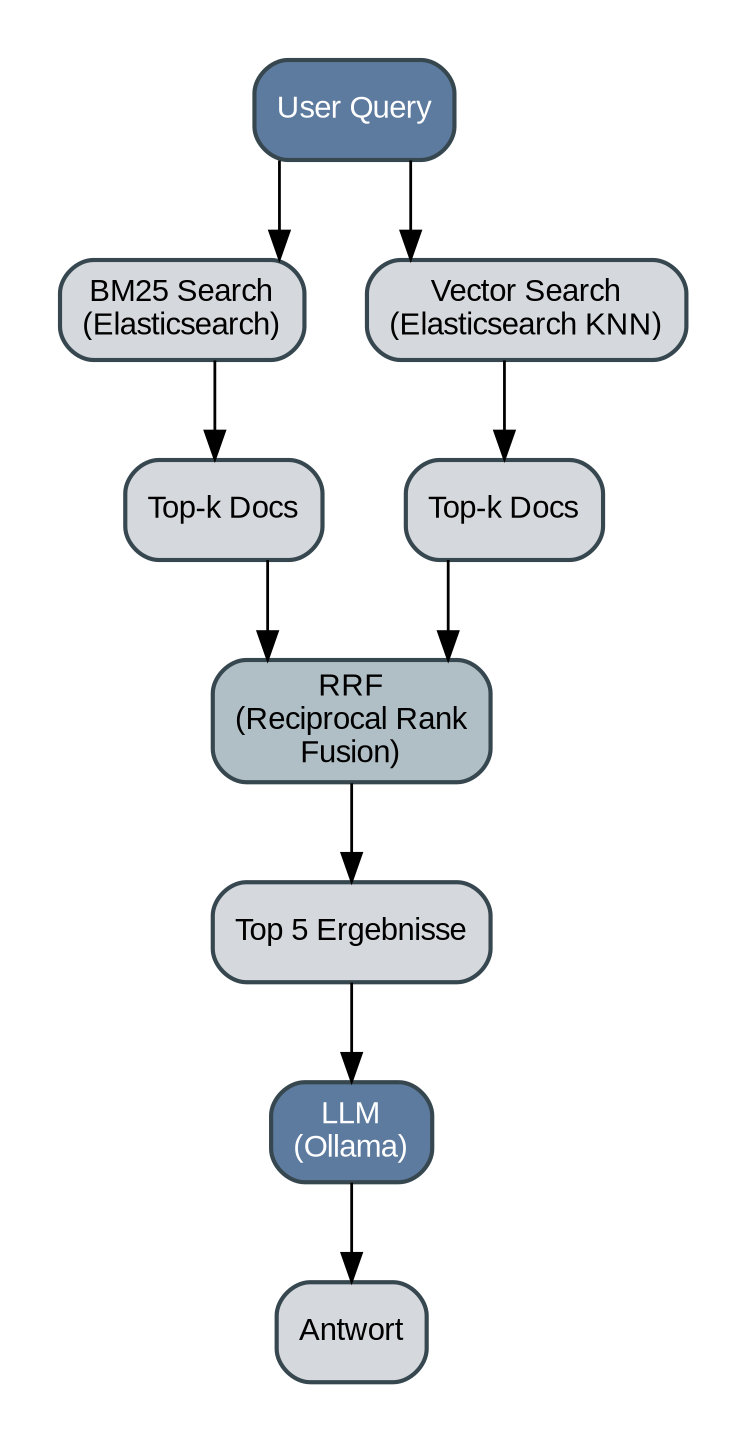
\includegraphics[width=0.8\textwidth]{Hybrid_Search.png}
\caption{Ablauf der hybriden Suche mit BM25, Vektorsuche und RRF}
\label{fig:hybrid}
\end{figure}

\clearpage

\subsection{Backend-Architektur mit FastAPI}

Das Backend wurde mit dem Framework FastAPI realisiert und fungiert als zentrale Orchestrierungsschicht des Systems. Es übernimmt die Verarbeitung eingehender Anfragen und koordiniert die Kommunikation zwischen den einzelnen Komponenten.

Dabei verbindet das Backend die Retrieval-Komponente (Elasticsearch), das Sprachmodell (über Ollama) sowie das Frontend.

\begin{lstlisting}[language=Python, caption={FastAPI Initialisierung}, label={lst:fastapi}]
app = FastAPI(
    title="RAG API - Bachelor Arbeit",
    version="1.0.0"
)

app.include_router(query_router, prefix="/api")
\end{lstlisting}

Zur Überprüfung der Systemverfügbarkeit wurde ein Health-Endpunkt implementiert:

\begin{lstlisting}[language=Python, caption={Health Endpoint}, label={lst:health}]
@app.get("/health")
async def health():
    return {"status": "healthy"}
\end{lstlisting}

Der Endpunkt \texttt{/api/ask} stellt die zentrale Schnittstelle dar und bildet den vollständigen RAG-Prozess ab.

\begin{figure}[h!]
\centering
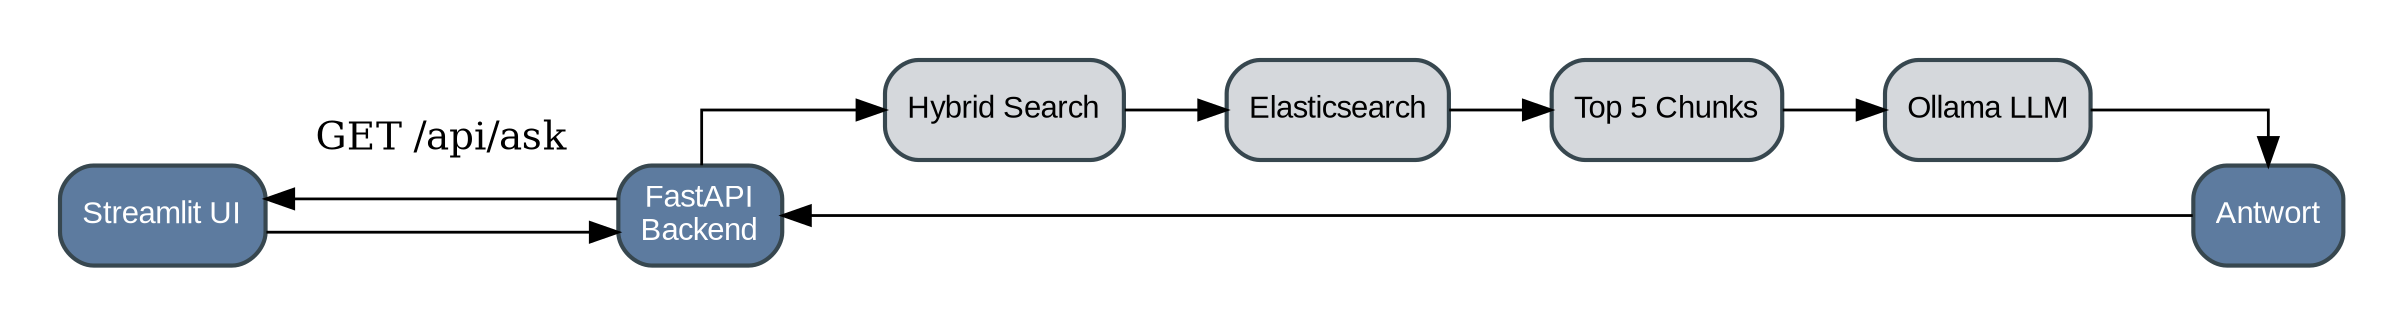
\includegraphics[width=1\textwidth]{API_Flow.png}
\caption{Ablauf einer Anfrage durch das Backend}
\label{fig:backend}
\end{figure}

\subsection{LLM-Integration und Prompting}

Die Generierung der Antworten erfolgt durch ein lokal betriebenes Large Language Model über die Ollama-Schnittstelle. Das Modell erhält sowohl die Nutzeranfrage als auch den zuvor ermittelten Kontext als Eingabe.

Das Sprachmodell verfügt über keinen direkten Zugriff auf externe Wissensquellen, sondern basiert ausschließlich auf dem bereitgestellten Kontext (Closed-Book-Ansatz).

Der Prompt wird dynamisch aufgebaut, um sicherzustellen, dass die Antwort ausschließlich auf den bereitgestellten Informationen basiert:

\begin{lstlisting}[language=Python, caption={Prompt-Erstellung}, label={lst:prompt}]
def build_prompt(query: str, context: str, intent: str, model: str) -> str:
    return f"""
KONTEXT:
{context}

FRAGE: {query}

Basiere deine Antwort nur auf dem Kontext.
"""
\end{lstlisting}

Diese Struktur trägt maßgeblich zur Reduktion von Halluzinationen bei und erhöht die Nachvollziehbarkeit der generierten Antworten.

\subsection{Antwortvalidierung}

Zur weiteren Verbesserung der Antwortqualität wurde ein zusätzlicher Validierungsschritt implementiert. Dabei wird überprüft, ob die generierte Antwort durch den bereitgestellten Kontext gestützt ist.

Die Validierung erfolgt durch eine modellbasierte Klassifikation der Antwort hinsichtlich ihrer Übereinstimmung mit dem Kontext.

\begin{lstlisting}[language=Python, caption={Faithfulness Check}, label={lst:faithfulness}]
def check_faithfulness(query: str, context: str, answer: str, model: str):
    if "JA" in verdict:
        return answer
    return FALLBACK_ANSWER
\end{lstlisting}

Falls die Antwort nicht ausreichend gestützt ist, wird eine alternative Antwort ausgegeben. Dieser Mechanismus reduziert das Risiko halluzinierter Inhalte.

\subsection{Frontend-Implementierung mit Streamlit}

Für die Benutzerinteraktion wurde ein webbasiertes Frontend mit Streamlit realisiert. Dieses ermöglicht die Eingabe natürlichsprachlicher Anfragen sowie die Darstellung der generierten Antworten in Form eines Chat-Interfaces.

Das Frontend dient ausschließlich der Interaktion und enthält keine Geschäftslogik, wodurch eine klare Trennung zwischen Präsentations- und Verarbeitungsschicht gewährleistet wird.

\begin{lstlisting}[language=Python, caption={Chat-Eingabe im Frontend}, label={lst:frontend}]
user_query = st.chat_input("Stellen Sie Ihre Frage")

if user_query:
    data = call_ask_api(user_query, selected_model)
\end{lstlisting}

\begin{figure}[h!]
\centering
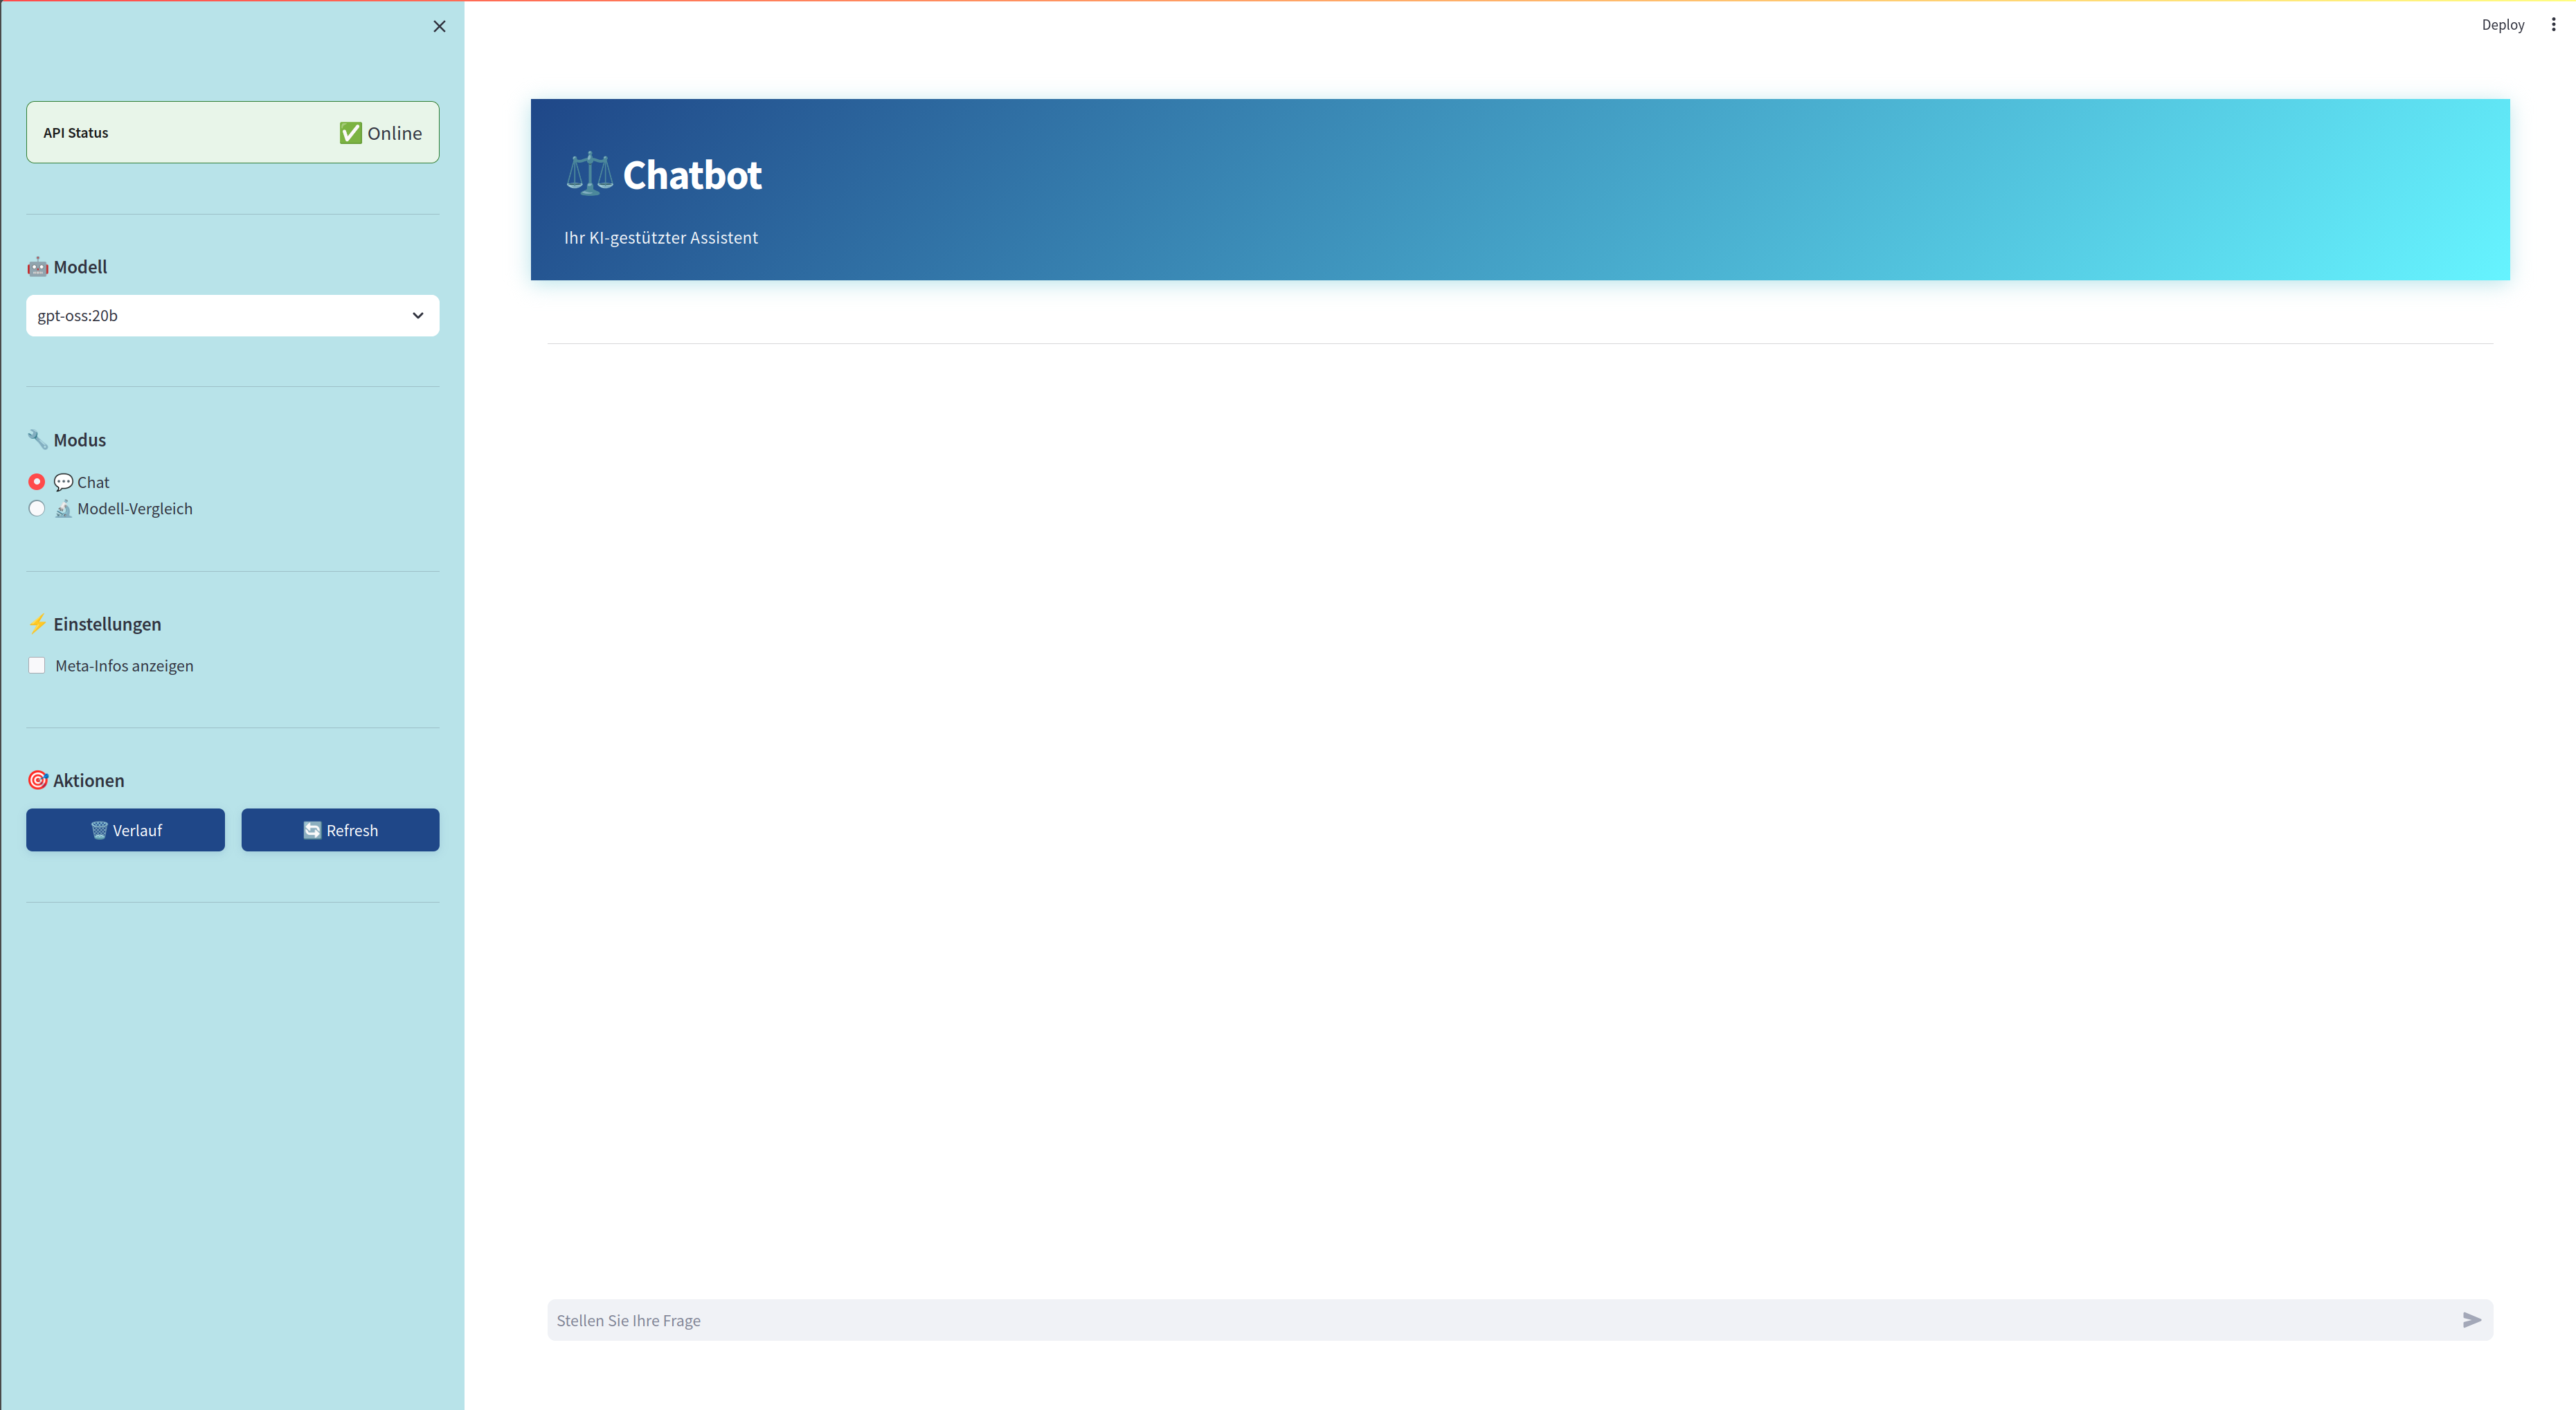
\includegraphics[width=0.9\textwidth]{frontend.png}
\caption{Benutzeroberfläche des Systems}
\label{fig:frontend}
\end{figure}

\subsection{Konfiguration}

Zentrale Systemparameter werden in einer Konfigurationsdatei definiert, um eine flexible Anpassung des Systems zu ermöglichen:

\begin{lstlisting}[language=Python, caption={Systemparameter}, label={lst:config}]
CHUNK_SIZE = 1000
HYBRID_BM25_W = 0.4
HYBRID_VECTOR_W = 0.6
\end{lstlisting}

Diese Parameter beeinflussen maßgeblich die Qualität der Suche sowie die Performance des Systems.

\subsection{Zusammenfassung}

Die Implementierung integriert Datenaufbereitung, hybride Suche, Backend-Architektur, Sprachmodellintegration sowie ein interaktives Frontend zu einem leistungsfähigen Gesamtsystem.

Die gewählte Architektur stellt einen Kompromiss zwischen Antwortqualität, Systemlatenz und Komplexität dar. Insbesondere die Kombination aus hybrider Suche und nachgelagerter Validierung trägt wesentlich zur Verbesserung der Ergebnisqualität bei und ermöglicht eine robuste, nachvollziehbare Verarbeitung natürlichsprachlicher Anfragen im Vergabekontext.

\clearpage
    \section{Evaluation}
\label{sec:Evaluation}

Ziel dieses Kapitels ist die systematische Bewertung des entwickelten Chatbots zur Unterstützung bei vergaberechtlichen Fragestellungen. Die Evaluation erfolgt auf zwei Ebenen: der Qualität der Dokumentenretrieval-Komponente sowie der Qualität der generierten Antworten. Hierfür werden sowohl klassische Information-Retrieval-Metriken als auch ein LLM-as-a-Judge-Ansatz eingesetzt.

\subsection{Evaluationsmethodik}

Die Evaluation basiert auf einem Datensatz realistischer Nutzeranfragen einschließlich der zugehörigen Referenzantworten sowie relevanter Ground-Truth-Dokumente. Ziel ist es, die Leistungsfähigkeit des entwickelten Retrieval-Augmented-Generation-(RAG)-Systems sowohl hinsichtlich der Dokumentensuche als auch der Antwortgenerierung systematisch zu bewerten.

Der Evaluationsaufbau orientiert sich an einem strukturierten Benchmark-Ansatz, um reproduzierbare und vergleichbare Ergebnisse zu gewährleisten. Hierzu werden die Anfragen in zwei Kategorien unterteilt: domänenspezifische, kontextbezogene Fragen aus dem Bereich des Vergaberechts sowie domänenfremde, kontextunabhängige Fragen. Diese Trennung ermöglicht eine differenzierte Analyse der fachlichen Antwortqualität sowie der Robustheit des Systems gegenüber irrelevanten oder außerhalb der Wissensbasis liegenden Eingaben.

Für jede Anfrage werden im Rahmen der Evaluation die folgenden Komponenten systematisch erfasst und gespeichert:
\begin{itemize}
    \item die ursprüngliche Nutzeranfrage,
    \item die durch das Retrieval-Modul identifizierten Dokumente,
    \item die generierte Antwort des Sprachmodells,
    \item sowie Referenzantworten bzw.\ relevante Ground-Truth-Dokumente.
\end{itemize}

Die Verarbeitung und Speicherung der Ergebnisse erfolgt in strukturierten JSON-Dateien. Dies ermöglicht eine automatisierte Auswertung sowie eine vollständige Nachvollziehbarkeit und Reproduzierbarkeit der Experimente.

Zur Bewertung des Systems kommen zwei komplementäre Ansätze zum Einsatz. Einerseits wird die Qualität des Retrievals mithilfe klassischer Information-Retrieval-Metriken wie Precision@k und Recall@k gemessen. Andererseits wird die Qualität der generierten Antworten durch einen LLM-as-a-Judge-Ansatz bewertet.

Die Antwortgenerierung erfolgt durch das Sprachmodell \textit{gpt-oss} (20B). Die Bewertung der generierten Antworten wird durch ein separates Sprachmodell (\textit{llama3.1:8b}) durchgeführt. Durch diese Trennung von Generierung und Bewertung wird eine methodisch fundierte und vergleichsweise objektive Einschätzung der Antwortqualität ermöglicht.

Der Datensatz umfasst unter anderem folgende Anfragen:

\textbf{Fragen im Kontext:}
\begin{enumerate}
    \item Ab welchem Betrag ist eine Vergabe durchzuführen (UVgO, VVÖA, LHO)?
    \item Ab welchem Betrag ist eine Beschaffung durchzuführen (UVgO, VVÖA, LHO)?
    \item Wie lange dauert ein Vergabeverfahren (UVgO, VgV)?
    \item Ist der Höchstbetrag in Brutto oder Netto anzugeben (UVgO, VgV, VVÖA)?
    \item Warum ist ein Vergabeverfahren durchzuführen (LHO, UVgO, VgV, VVÖA)?
    \item Welcher Preis ist zu beachten (VV~ÖA)?
    \item Als Mitarbeitender oder Professorin möchte ich wissen, ob Beträge, Preise und Kostenschätzungen in Brutto oder Netto anzugeben sind, um das korrekte Verfahren bestimmen zu können.
    \item Als Institutssekretariat möchte ich wissen, welche Dokumente der Beschaffungsstelle vorgelegt werden müssen, um eine Bestellung rechtssicher einzuleiten.
    \item Als wissenschaftlich Mitarbeitender möchte ich wissen, wie lange eine Ausschreibung offen sein muss und welche Fristen für Angebotsabgabe und Zuschlag gelten.
    \item Als wissenschaftlich Mitarbeitende möchte ich erfahren, ob Angebote selbst eingeholt werden dürfen oder ob dies durch die Beschaffungsstelle erfolgt.
    \item Als Projektleiterin oder Mitarbeitender möchte ich verstehen, was ein Vergabeverfahren bzw.\ eine Beschaffung im Kontext der Vergaberegelungen bedeutet.
    \item Als Projektleiter*in einer rheinland-pfälzischen Hochschule möchte ich wissen, warum Vergabeverfahren durchgeführt werden müssen und warum eine direkte Vergabe an einen Wunschlieferanten nicht zulässig ist.
\end{enumerate}

\textbf{Fragen außerhalb des Kontexts:}
\begin{enumerate}
    \item Wie mache ich eine Mondlandung?
    \item Wie koche ich Pasta?
    \item Wer hat die Relativitätstheorie erfunden?
    \item Wie repariere ich einen kaputten Laptop?
    \item d
\end{enumerate}

Durch die Kombination aus Retrieval-Evaluation und LLM-basierter Antwortbewertung wird ein ganzheitliches Benchmarking des Systems entlang der gesamten RAG-Pipeline ermöglicht. Dies erlaubt sowohl die isolierte Analyse einzelner Komponenten als auch die Untersuchung ihrer Wechselwirkungen innerhalb der Gesamtarchitektur.

\subsection{Bewertungsmetriken}

Zur Bewertung wurden zwei zentrale Ansätze verwendet:

\textbf{Klassische Information-Retrieval-Metriken (Precision@k, Recall@k)}\
Diese Metriken messen die Qualität der Dokumentensuche. Precision@k gibt an, wie viele der Top- k  zurückgegebenen Dokumente relevant sind, während Recall@k den Anteil der insgesamt relevanten Dokumente misst, der in den Top- k  enthalten ist. Die Relevanz wurde zweistufig definiert:
\begin{itemize}
    \item \textit{Mode A (streng)}: Nur Dokumente mit \texttt{relevanz=hoch} gelten als relevant.
    \item \textit{Mode B (moderat)}: Dokumente mit \texttt{relevanz=hoch} oder \texttt{relevanz=mittel} gelten als relevant.
\end{itemize}

\textbf{LLM-basierte Bewertung der Antwortqualität (LLM-as-a-Judge)}\
Für die Bewertung der Antwortqualität wurde ein lokal ausgeführtes LLM (\texttt{llama3.1:8b}) verwendet. Das Modell fungiert als unabhängiger Gutachter und bewertet die generierten Antworten auf Basis eines strukturierten Prompts anhand von vier Kriterien auf einer Skala von 1 (schlecht) bis 5 (sehr gut):

\begin{description}
    \item[Correctness (Korrektheit):] Ist die Antwort fachlich korrekt basierend auf den Quellen?
    \item[Completeness (Vollständigkeit):] Beantwortet die Antwort die Frage vollständig?
    \item[Faithfulness (Faktentreue):] Bleibt die Antwort treu zu den gegebenen Quellen (keine Halluzinationen)?
    \item[Clarity (Klarheit):] Ist die Antwort klar, strukturiert und verständlich?
\end{description}

Durch den Einsatz eines separaten Modells wird eine objektivere Einschätzung der Antwortqualität ermöglicht, da die Bewertung unabhängig vom generierenden System erfolgt.

Die Ergebnisse wurden in JSON-Dateien gespeichert und anschließend automatisiert ausgewertet. Die Auswertung erfolgt getrennt für Kontextfragen und Out-of-Context-Fragen, um ein differenziertes Bild der Systemleistung zu erhalten.

\subsection{Retrieval-Evaluation}

Zur Bewertung der Suchqualität werden die Metriken Precision@k und Recall@k herangezogen. Diese quantifizieren den Anteil relevanter Dokumente innerhalb der Top- k -Ergebnisse sowie die Abdeckung aller relevanten Dokumente.

\begin{itemize}
    \item Precision@k = relevante Treffer in Top- k  /  k 
    \item Recall@k = relevante Treffer in Top- k  / Gesamtanzahl relevanter Dokumente
\end{itemize}

Die dargestellten Ergebnisse basieren auf aggregierten Durchschnittswerten über mehrere evaluierte Anfragen. Für jeden  k -Wert wurden Precision und Recall über alle betrachteten Fragen gemittelt, um eine vergleichbare Bewertung der Retrieval-Leistung zu ermöglichen.

Die Ergebnisse für die In-Context-Fragen weisen auf eine sehr hohe Retrieval-Qualität hin. Über alle betrachteten  k -Werte hinweg erreicht das System eine konstante Precision von 1{,}0, was bedeutet, dass ausschließlich relevante Dokumente unter den Top- k -Ergebnissen enthalten sind.

Der Recall steigt mit zunehmendem  k  kontinuierlich an. Während bei  k=1  lediglich ein kleiner Teil der relevanten Dokumente identifiziert wird (Recall@1 = 0{,}07), erhöht sich die Abdeckung sukzessive. Bei  k=10  werden bereits rund zwei Drittel der relevanten Dokumente gefunden, und bei  k=15  wird schließlich ein vollständiger Recall von 1{,}0 erreicht. Dies deutet darauf hin, dass relevante Dokumente zuverlässig im Ranking enthalten sind, jedoch nicht immer auf den obersten Positionen erscheinen.

\begin{figure}[H]
\centering
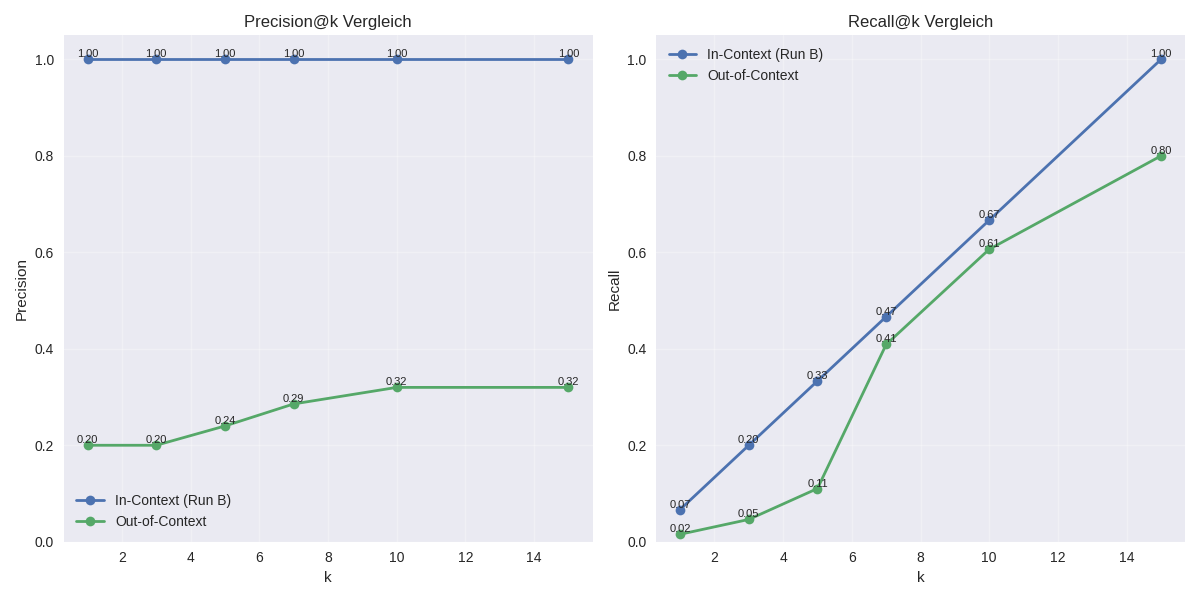
\includegraphics[width=0.9\textwidth]{precrecall.png}
\caption{Precision@k und Recall@k für verschiedene Werte von  k  (Vergleich von In-Context- und Out-of-Context-Fragen)}
\label{fig:precision_recall1}
\end{figure}

Im Gegensatz dazu weisen die Ergebnisse für die Out-of-Context-Fragen auf eine deutlich geringere Retrieval-Qualität hin. Die Precision liegt bei kleinen  k -Werten bei etwa 0{,}20 und steigt nur moderat auf rund 0{,}32 bei größeren  k -Werten. Dies verdeutlicht, dass ein erheblicher Anteil der zurückgegebenen Dokumente nicht relevant ist.

Auch der Recall ist für Out-of-Context-Anfragen zunächst sehr gering (Recall@1 = 0{,}02), steigt jedoch mit wachsendem  k  deutlich an und erreicht bei  k=15  einen Wert von etwa 0{,}80. Dieser Anstieg ist jedoch mit einer vergleichsweise niedrigen Precision verbunden, was darauf hinweist, dass relevante Dokumente erst durch eine größere Anzahl zusätzlicher, teilweise irrelevanter Treffer gefunden werden.

Insgesamt weisen die Ergebnisse darauf hin, dass die Retrieval-Leistung vom Kontext der Anfrage beeinflusst wird. Während In-Context-Fragen mit hoher Präzision und wachsendem Recall beantwortet werden können, führt das Fehlen eines passenden Kontexts bei Out-of-Context-Anfragen zu einer geringeren Ergebnisqualität.

\clearpage
\subsubsection{Analyse der Hybrid-Suche}

Die Analyse des Überlappungsgrades zwischen BM25 und Vektorsuche zeigt insgesamt eine geringe Überschneidung der identifizierten Dokumente und verdeutlicht die unterschiedlichen Eigenschaften beider Retrieval-Ansätze.

Für die In-Context-Anfrage zeigt sich eine teilweise Überschneidung der Ergebnisse. Wie in Abbildung~\ref{fig:bm25_vector_in} dargestellt, werden drei Dokumente von beiden Verfahren identifiziert, was einem Überlappungsgrad von etwa 23,% entspricht. Gleichzeitig existieren mehrere Dokumente, die ausschließlich von einem der beiden Verfahren gefunden werden.

Dies verdeutlicht die komplementären Eigenschaften der Ansätze: Während BM25 auf exakten Termübereinstimmungen basiert, erfasst die Vektorsuche semantische Zusammenhänge. Die Kombination beider Verfahren ermöglicht somit eine breitere Abdeckung relevanter Dokumente.

\begin{figure}[H]
    \centering
    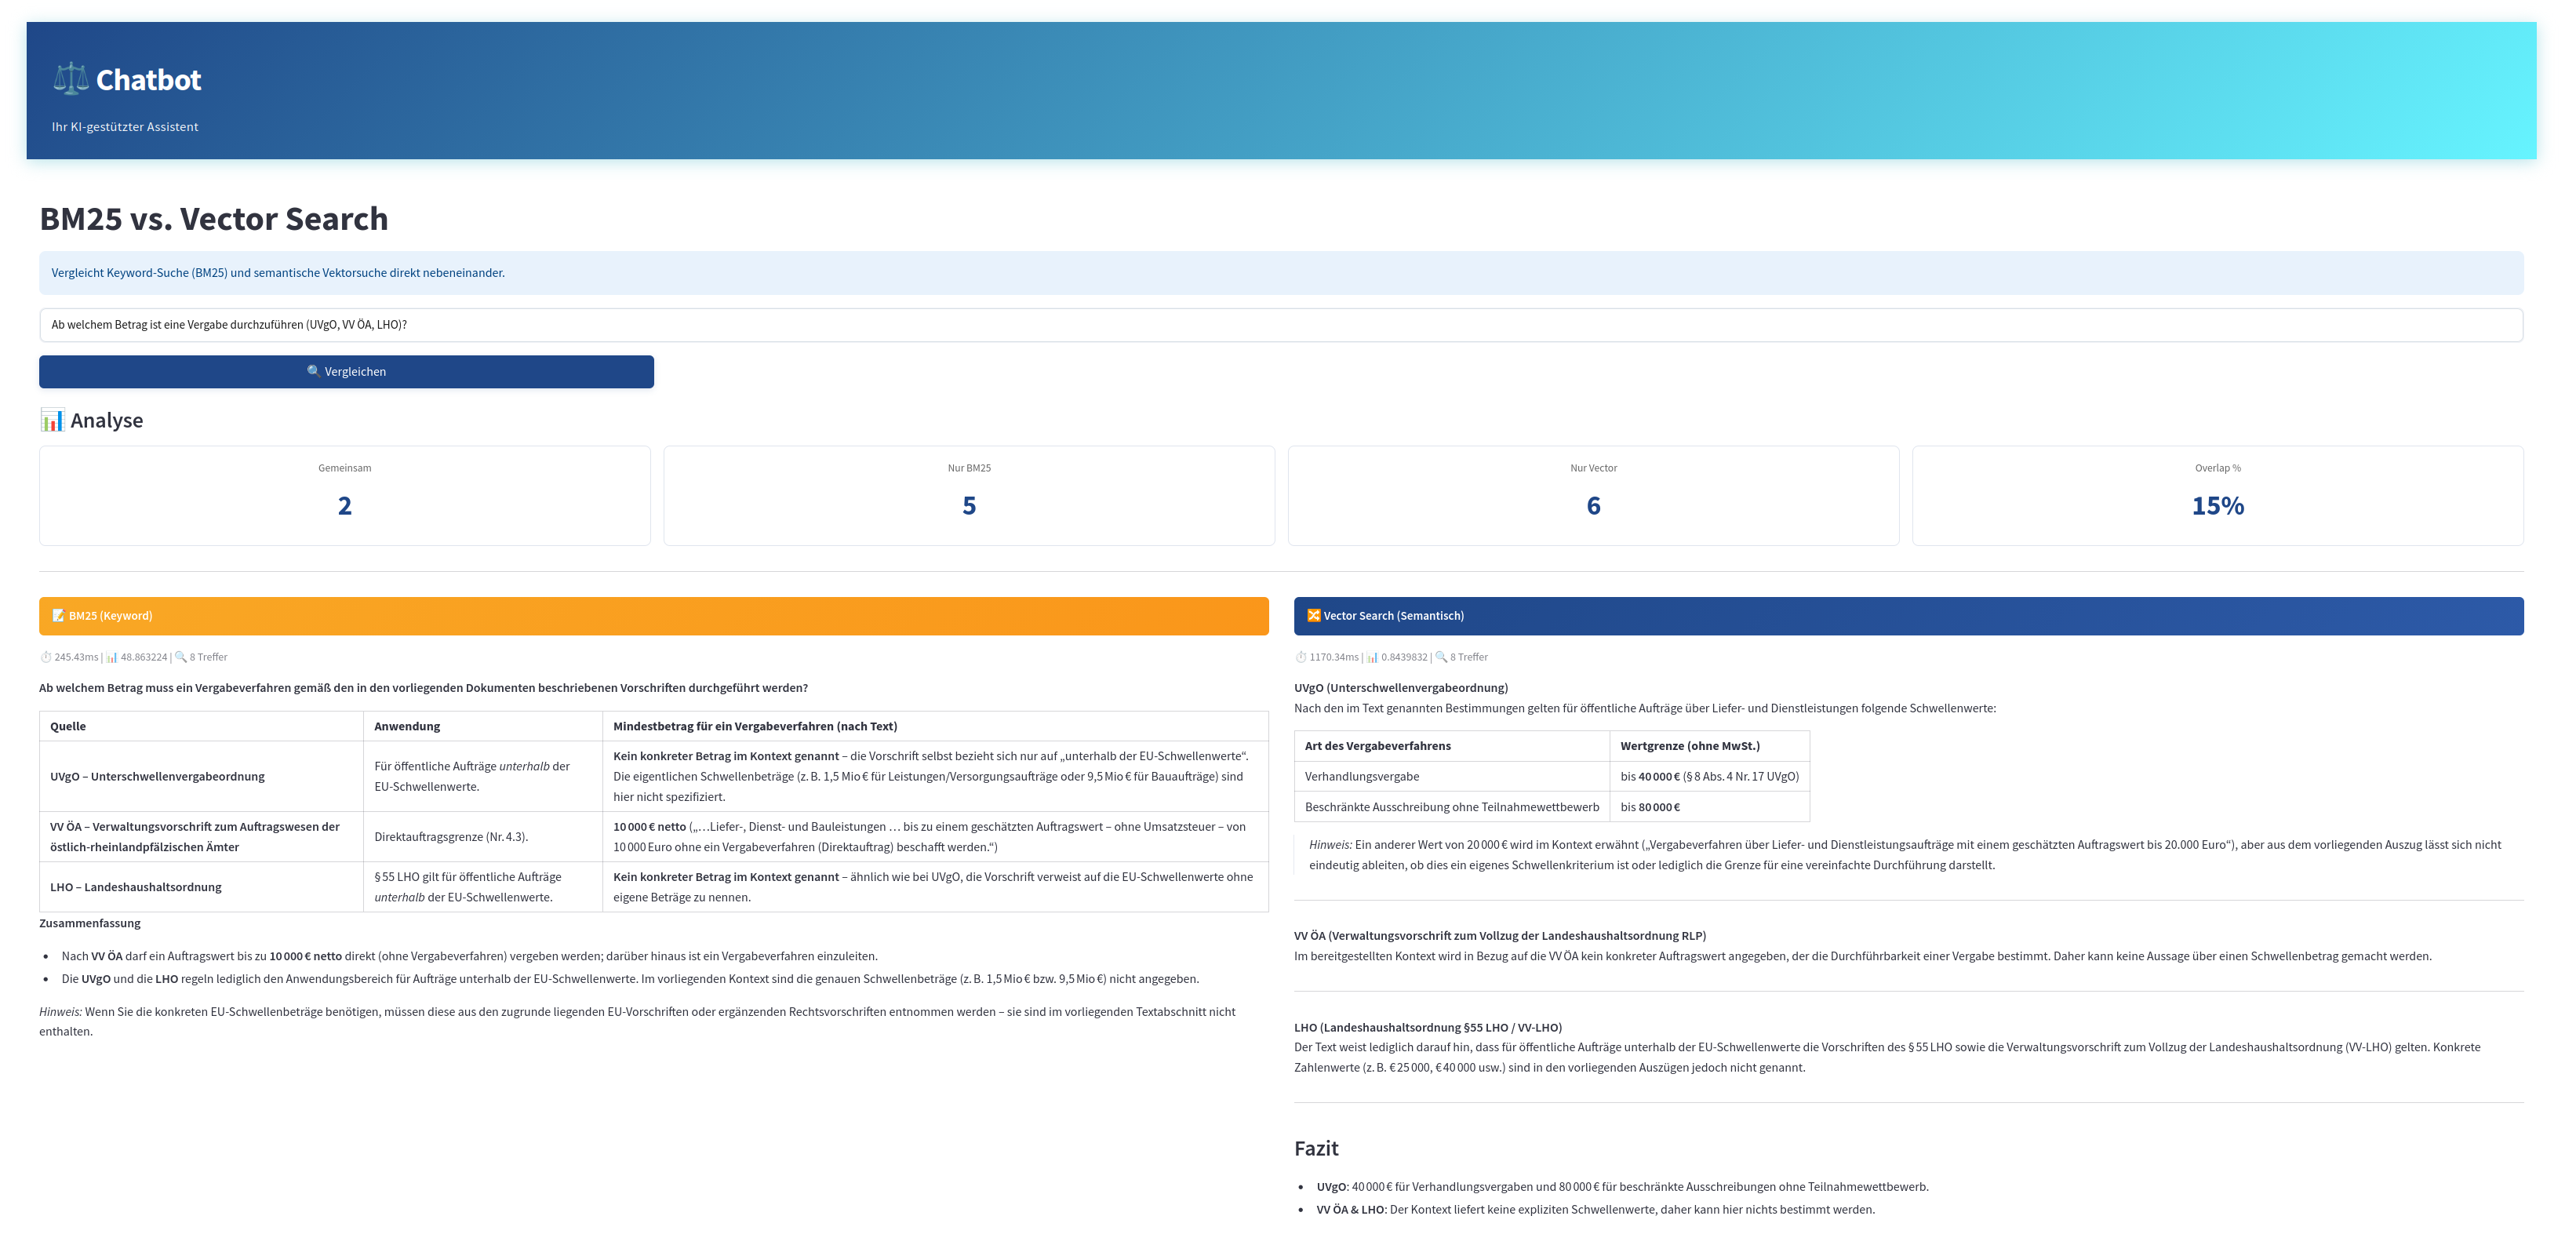
\includegraphics[width=0.9\textwidth]{Vergleich_BM25_Vector.png}
    \caption{Vergleich der Retrieval-Ergebnisse von BM25 und Vektorsuche für eine In-Context-Anfrage ( k=5 )}
    \label{fig:bm25_vector_in}
\end{figure}

Im Gegensatz dazu zeigt die Out-of-Context-Anfrage eine vollständige Divergenz der Ergebnisse. Wie in Abbildung~\ref{fig:bm25_vector_out} zu sehen ist, existiert keine Überschneidung zwischen den von BM25 und der Vektorsuche identifizierten Dokumenten (0,\%).

Dieses Verhalten unterstreicht die unterschiedlichen Suchprinzipien besonders deutlich: Ohne passenden Kontext greifen die Verfahren auf verschiedene, jeweils nicht optimal geeignete Relevanzsignale zurück.

\begin{figure}[H]
    \centering
    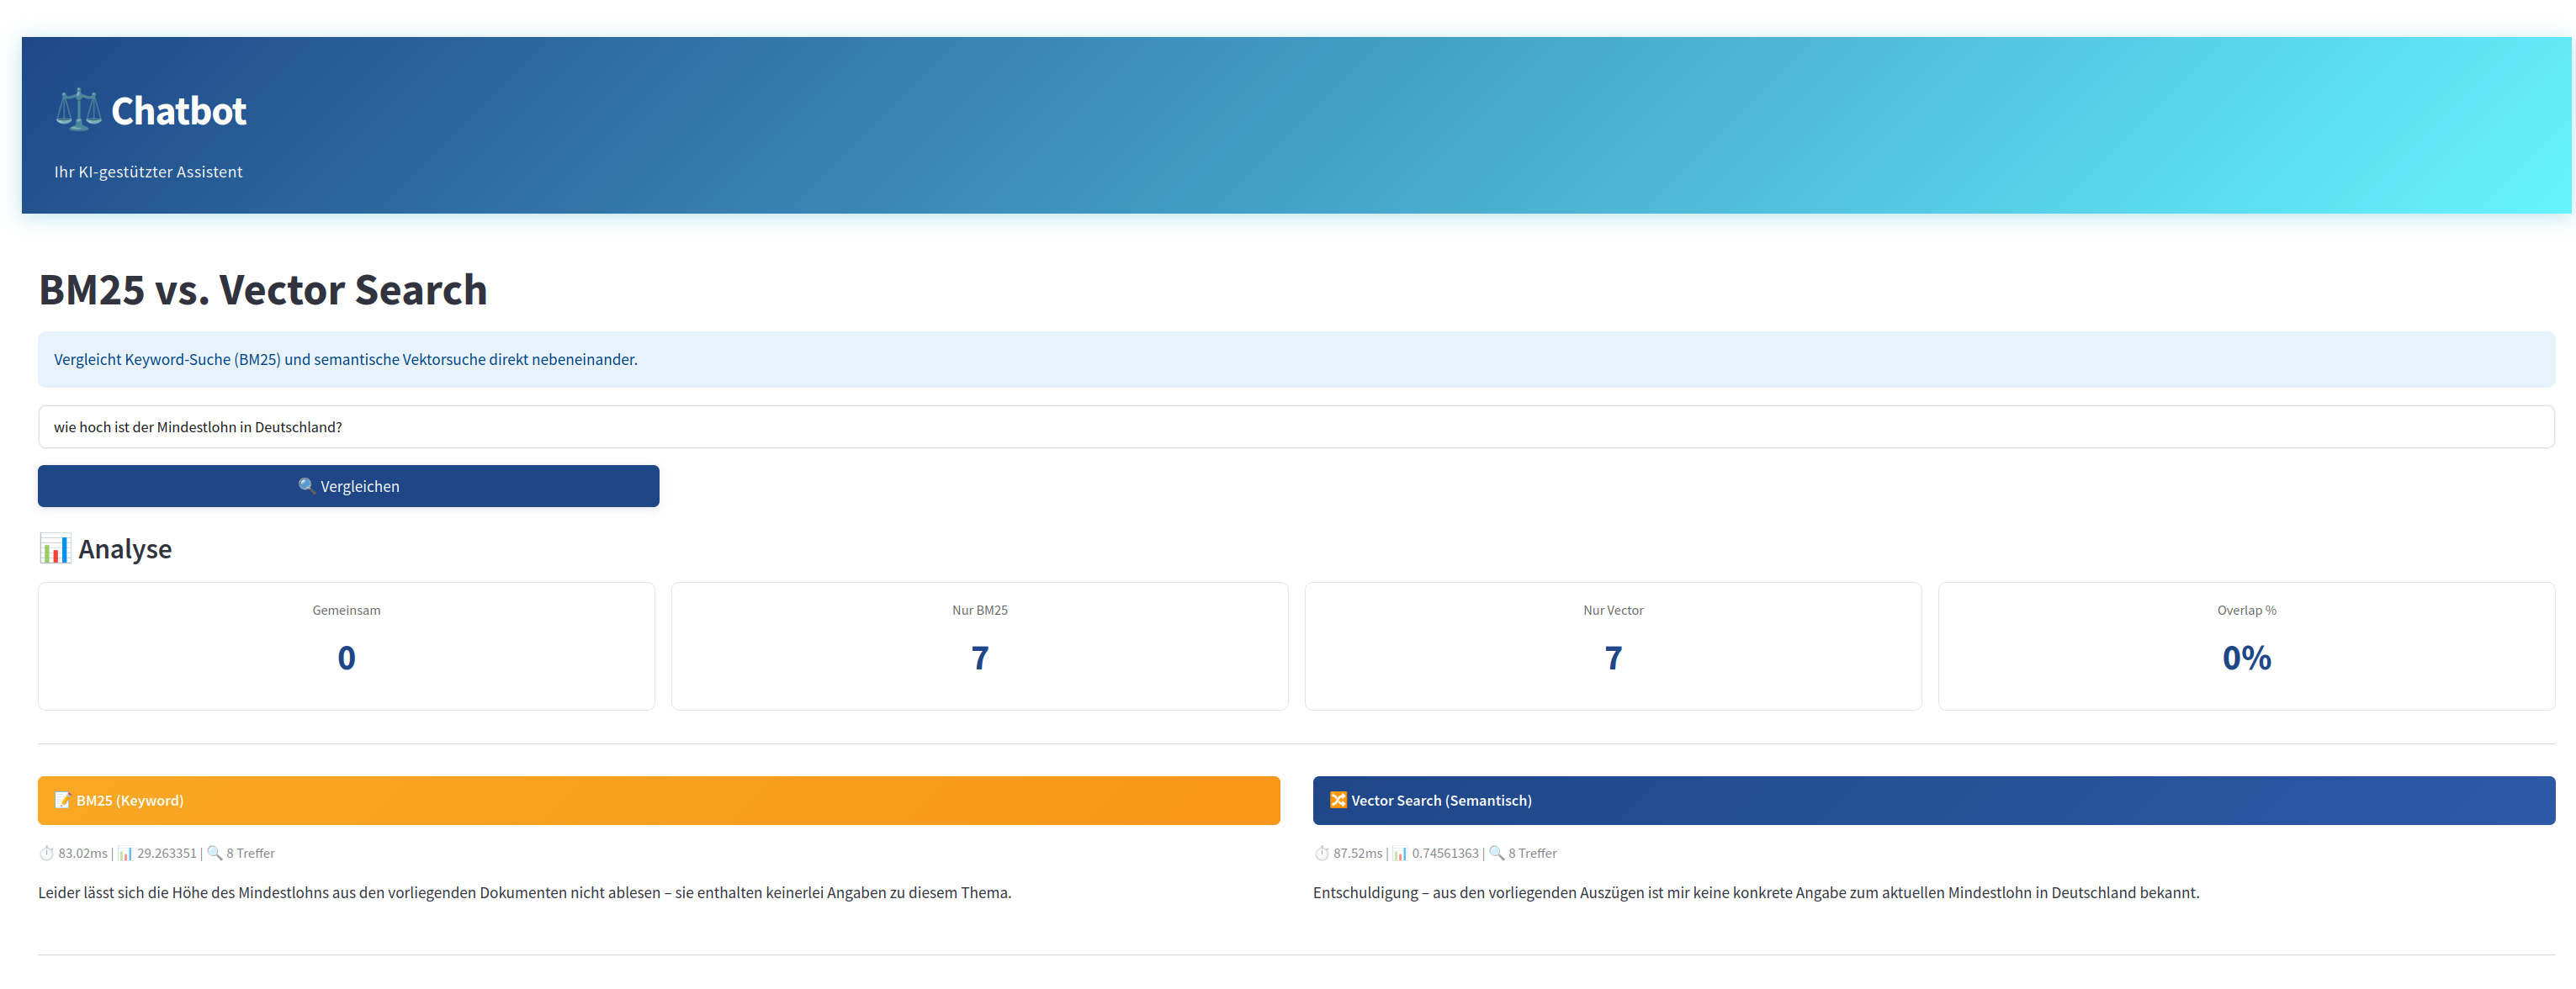
\includegraphics[width=0.9\textwidth]{out_bm25_vector.png}
    \caption{Vergleich der Retrieval-Ergebnisse von BM25 und Vektorsuche für eine Out-of-Context-Anfrage ( k=5 )}
    \label{fig:bm25_vector_out}
\end{figure}

Insgesamt legen die Ergebnisse nahe, dass BM25 und Vektorsuche komplementäre Eigenschaften aufweisen und ihre Kombination zu einer verbesserten Abdeckung relevanter Dokumente beitragen kann.

\subsection{Ergebnisse der Antwortbewertung}

Zur Bewertung der generierten Antworten wird ein LLM-as-a-Judge-Ansatz eingesetzt. Die Antworten werden durch das Modell \textit{gpt-oss} (20B) generiert und anschließend durch \textit{llama3.1:latest} bewertet.

Die Bewertung erfolgt anhand der folgenden Kriterien:

\begin{itemize}
    \item Correctness (fachliche Korrektheit)
    \item Completeness (inhaltliche Vollständigkeit)
    \item Faithfulness (Quellentreue)
    \item Clarity (Verständlichkeit und Struktur)
\end{itemize}

Die dargestellten Ergebnisse basieren auf aggregierten Durchschnittswerten über mehrere evaluierte Fragen. Für jede Kategorie wurde der arithmetische Mittelwert der durch das LLM vergebenen Bewertungen berechnet, um eine vergleichbare Gesamtbewertung der Antwortqualität zu ermöglichen.

Die Ergebnisse werden getrennt für In-Context- und Out-of-Context-Fragen betrachtet.

Für die In-Context-Fragen zeigt sich ein insgesamt hohes Qualitätsniveau:

\begin{itemize}
    \item Correctness: 4{,}75
    \item Completeness: 4{,}33
    \item Faithfulness: 4{,}33
    \item Clarity: 4{,}67
\end{itemize}

Dies entspricht einer Gesamtbewertung von 4{,}52 von 5{,}0 Punkten (vgl. Abbildung~\ref{fig:judge_scores_in}).

\begin{figure}[h]
    \centering
    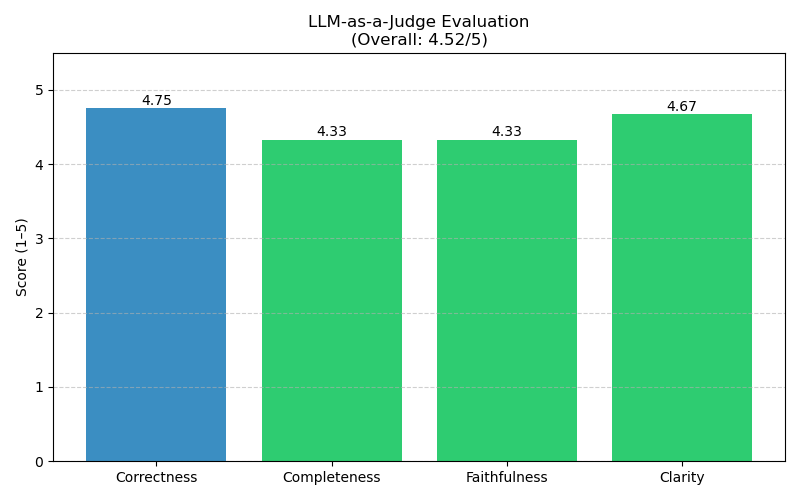
\includegraphics[width=0.75\textwidth]{judge_scores_in_context.png}
    \caption{LLM-basierte Bewertung der Antwortqualität für In-Context-Fragen}
    \label{fig:judge_scores_in}
\end{figure}

Die Ergebnisse zeigen, dass die generierten Antworten überwiegend fachlich korrekt, klar strukturiert und eng an den zugrunde liegenden Quellen orientiert sind. Leichte Abweichungen zeigen sich insbesondere bei der Vollständigkeit und Quellentreue.

Für Out-of-Context-Fragen ergibt sich hingegen ein deutlich geringerer Gesamtscore:

\begin{itemize}
    \item Correctness: 2{,}80
    \item Completeness: 2{,}60
    \item Faithfulness: 5{,}00
    \item Clarity: 4{,}40
\end{itemize}

Dies entspricht einer Gesamtbewertung von 3{,}70 von 5{,}0 Punkten (vgl. Abbildung~\ref{fig:judge_scores_out}).

\begin{figure}[h]
    \centering
    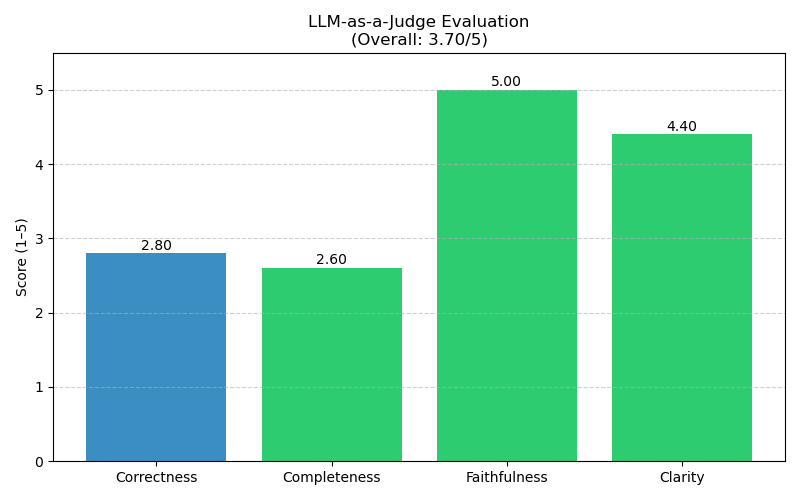
\includegraphics[width=0.75\textwidth]{judge_scores_out_context.png}
    \caption{LLM-basierte Bewertung der Antwortqualität für Out-of-Context-Fragen}
    \label{fig:judge_scores_out}
\end{figure}

Auffällig ist insbesondere die konstant hohe Bewertung der Faithfulness bei Out-of-Context-Fragen. Dies deutet darauf hin, dass das System keine nicht durch den Kontext gestützten Informationen generiert und somit ein robustes Verhalten gegenüber Halluzinationen aufweist.

Es ist jedoch zu beachten, dass durch die Verwendung von Durchschnittswerten individuelle Abweichungen einzelner Antworten nicht im Detail sichtbar werden. Die Ergebnisse liefern daher primär eine aggregierte Einschätzung der Systemleistung.

Insgesamt verdeutlichen die Ergebnisse, dass die Qualität der generierten Antworten maßgeblich von der Verfügbarkeit relevanter Kontextinformationen abhängt.

\subsubsection{Qualitative Analyse}

Die qualitative Analyse zeigt zwei zentrale Verhaltensweisen des Systems.

Zum einen erkennt das System Situationen, in denen die bereitgestellten Kontextinformationen nicht ausreichen, und kommuniziert diese Unsicherheit explizit. Dieses Verhalten trägt zur Reduktion von Halluzinationen bei.

Zum anderen werden in Einzelfällen zusätzliche Informationen generiert, die nicht vollständig durch die zugrunde liegenden Quellen abgesichert sind. Dies verdeutlicht die inhärenten Grenzen des Systems im Umgang mit unvollständigem Kontext.

\subsection{Diskussion}

Die Kombination aus Retrieval-Metriken und LLM-basierter Bewertung ermöglicht eine differenzierte Analyse der Systemleistung.

Während Precision@k und Recall@k die Effektivität der Dokumentensuche quantifizieren, bewertet der LLM-as-a-Judge-Ansatz die Nutzbarkeit der generierten Antworten auf Basis aggregierter Durchschnittswerte.

Die Ergebnisse deuten darauf hin, dass die hybride Suche zur Verbesserung der Retrieval-Abdeckung beiträgt, indem unterschiedliche Stärken von BM25 und Vektorsuche kombiniert werden.

Zudem zeigt sich ein Zusammenhang zwischen der Qualität der Retrieval-Ergebnisse und der Qualität der generierten Antworten. Insbesondere bei fehlendem oder unzureichendem Kontext sinkt die Antwortqualität.

Die beobachteten Einschränkungen in der Vollständigkeit können im Kontext der verwendeten RAG-Architektur interpretiert werden und stehen im Zusammenhang mit der Verfügbarkeit relevanter Dokumente.

\subsection{Zusammenfassung}

Zusammenfassend lässt sich festhalten, dass das entwickelte System in den durchgeführten Evaluationsszenarien insgesamt gute Ergebnisse erzielt.

Die Hybrid-Suche ermöglicht die zuverlässige Identifikation relevanter Dokumente und erreicht bei höheren  k -Werten einen vollständigen Recall. Die generierten Antworten weisen insgesamt eine hohe fachliche Qualität sowie eine ausgeprägte Quellentreue auf.

Einschränkend ist anzumerken, dass der Evaluationsdatensatz mit drei Testfragen nur eine begrenzte Aussagekraft besitzt. Zudem können durch die Verwendung von Durchschnittswerten individuelle Abweichungen einzelner Bewertungen nicht vollständig abgebildet werden.

Eine Erweiterung des Datensatzes sowie die Einbeziehung menschlicher Evaluationen stellen sinnvolle Ansätze für zukünftige Arbeiten dar.

Insgesamt legen die Ergebnisse nahe, dass die Kombination aus Hybrid-Retrieval und LLM-basierter Antwortgenerierung eine geeignete Grundlage für ein domänenspezifisches Expertensystem im vergaberechtlichen Kontext darstellen kann.
\clearpage
    \section{Diskussion}
\label{sec:Diskussion}

Aufbauend auf den Ergebnissen der Evaluation erfolgt im Folgenden eine übergeordnete Einordnung und kritische Reflexion des entwickelten Systems.

Die durchgeführten Experimente zeigen, dass das vorgestellte Retrieval-Augmented-Generation-System grundsätzlich in der Lage ist, vergaberechtliche Fragestellungen mit hoher Qualität zu beantworten, sofern relevante Kontextinformationen verfügbar sind. Insbesondere die Ergebnisse der In-Context-Evaluation verdeutlichen, dass sowohl die Dokumentensuche als auch die darauf basierende Antwortgenerierung zuverlässig funktionieren.

Ein zentrales Ergebnis der Arbeit ist die beobachtete Wirksamkeit des hybriden Retrieval-Ansatzes. Die Kombination aus BM25 und Vektorsuche ermöglicht es, sowohl lexikalische Übereinstimmungen als auch semantische Zusammenhänge zu berücksichtigen. Die geringe Überschneidung der jeweils gefundenen Dokumente deutet darauf hin, dass beide Verfahren unterschiedliche Aspekte von Relevanz erfassen und sich somit sinnvoll ergänzen. In der Gesamtbetrachtung führt dies zu einer verbesserten Abdeckung relevanter Dokumente im Vergleich zu einzelnen Retrieval-Ansätzen.

Gleichzeitig wird deutlich, dass die Qualität der generierten Antworten maßgeblich von der Qualität der Retrieval-Ergebnisse abhängt. Diese enge Kopplung ist charakteristisch für RAG-Systeme und stellt eine zentrale Limitation dar: Unvollständige oder nicht optimal gerankte Dokumente wirken sich unmittelbar auf die Antwortqualität aus. Die in der Evaluation beobachteten Einschränkungen hinsichtlich der Vollständigkeit lassen sich vor diesem Hintergrund plausibel erklären.

Die Ergebnisse der Out-of-Context-Evaluation verdeutlichen zudem die Grenzen des Systems. Ohne geeignete Kontextgrundlage sinkt die Qualität der generierten Antworten signifikant. Gleichzeitig zeigt sich jedoch ein positives Verhalten im Hinblick auf die Vermeidung von Halluzinationen: Das System tendiert dazu, Unsicherheiten zu erkennen und entsprechend zurückhaltend zu reagieren, anstatt nicht fundierte Informationen zu generieren. Dieses Verhalten ist insbesondere im juristischen Anwendungskontext von hoher Relevanz, da die Verlässlichkeit der bereitgestellten Informationen eine zentrale Anforderung darstellt.

Neben den Stärken des Systems sind auch mehrere Limitationen zu berücksichtigen. Die Aussagekraft der Evaluation ist durch die begrenzte Größe des Datensatzes eingeschränkt. Insbesondere kann die Verwendung weniger Testfragen dazu führen, dass bestimmte Fehlermuster oder Randfälle nicht ausreichend erfasst werden. Darüber hinaus basiert die Bewertung der Antwortqualität auf einem LLM-as-a-Judge-Ansatz, der trotz strukturierter Bewertungskriterien keine vollständig objektive Beurteilung ersetzen kann.

Ein weiterer Aspekt betrifft die Aggregation der Ergebnisse über Durchschnittswerte. Diese ermöglicht zwar eine kompakte Darstellung der Gesamtleistung, kann jedoch individuelle Abweichungen und spezifische Schwächen einzelner Antworten überdecken. Für eine detailliertere Analyse wäre daher eine ergänzende fallbasierte Betrachtung sinnvoll.

Im Kontext verwandter Arbeiten ordnen sich die Ergebnisse in bestehende Erkenntnisse zu Retrieval-Augmented-Generation-Systemen ein. Insbesondere bestätigt sich die zentrale Rolle des Retrievals als limitierender Faktor für die Gesamtleistung sowie der Nutzen hybrider Suchansätze zur Verbesserung der Dokumentenabdeckung.

Für zukünftige Arbeiten ergeben sich mehrere Ansatzpunkte. Eine Erweiterung des Evaluationsdatensatzes sowie die Einbeziehung menschlicher Expertinnen und Experten in den Bewertungsprozess könnten die Aussagekraft der Ergebnisse deutlich erhöhen. Darüber hinaus erscheint die Optimierung des Retrieval-Rankings, beispielsweise durch Re-Ranking-Strategien oder domänenspezifisches Fine-Tuning, als vielversprechender Ansatz zur weiteren Steigerung der Systemleistung.

Insgesamt zeigen die Ergebnisse, dass das entwickelte System eine solide Grundlage für ein domänenspezifisches Assistenzsystem im vergaberechtlichen Kontext darstellt, gleichzeitig jedoch weitere Optimierungspotenziale bestehen.
\clearpage
    \section{Fazit und Ausblick} 
\subsection{Fazit}
Die Untersuchung hatte zum Ziel, die Anwendbarkeit von Large Language Models (LLMs) in einem thematisch fokussierten Expertensystem zusammen mit hybriden Retrieval-Methoden zu bewerten. Ein Retrieval-Augmented-Generation-(RAG)-System wurde hierfür entwickelt, das eine BM25-basierte Volltextsuche mit einer semantischen Vektorsuche innerhalb von Elasticsearch kombiniert und die ermittelten Informationen zur kontextuellen Antwortgenerierung an ein Large Language Model übergibt.  

Die Evaluationsergebnisse belegen, dass die Antwortqualität erheblich verbessert werden kann, wenn man Retrieval-Mechanismen und LLMs kombiniert. Gerade das Einfügen von relevanten Textabschnitten erlaubt es, die Generierung stärker zu steuern und verbessert die inhaltliche Nachvollziehbarkeit der Antworten. So kann das Risiko von Halluzinationen verringert werden, obwohl es nicht gänzlich ausgeschlossen werden kann.  

Eine hybride Suchstrategie hat sich als besonders wirkungsvoll erwiesen, weil sie einerseits exakte Treffer durch lexikalische Verfahren und andererseits semantisch ähnliche Inhalte umfasst. Eine bessere Trefferqualität im Retrieval-Schritt ist das Ergebnis dessen, was wiederum eine entscheidende Grundlage für die Qualität der generierten Antworten ist.  

Die Arbeit demonstriert zudem, dass ein solches System domänenspezifisches Wissen aus großen Dokumentensammlungen effizient zugänglich macht und nutzerfreundlich aufbereitet.  Dies bietet einen erheblichen Vorteil, besonders wenn es um komplizierte Regelungen wie die im Vergaberecht geht.  

Es wird jedoch auch offensichtlich, dass die Effizienz des Systems stark von der Qualität der zugrunde liegenden Daten, der ausgewählten Retrieval-Strategie und der Gestaltung der Prompt abhängt.  Um sicherzustellen, dass die Ergebnisse verlässlich sind, ist es unerlässlich, das System sorgfältig zu konzipieren. 

Es ist festzustellen, dass die Nutzung von Large Language Models zusammen mit hybriden Retrieval-Methoden grundsätzlich sinnvoll und umsetzbar ist, um die Forschungsfrage zu beantworten. Vor allem, wenn man datengestütztes Retrieval mit generativer Sprachverarbeitung kombiniert, kann man die Qualität, Nachvollziehbarkeit und Relevanz der Antworten erheblich verbessern.  

Alles in allem ist Retrieval-Augmented-Generation ein vielversprechender Ansatz für den Einsatz von Large Language Models in Expertensystemen und bietet eine praktikable Möglichkeit, die Vorzüge datengetriebener Sprachmodelle mit strukturierten Wissensquellen zu vereinen.
\subsection{Einschränkungen}
Obwohl die Ergebnisse positiv sind, hat das entwickelte System einige Einschränkungen. Eine wesentliche Herausforderung bleibt die Möglichkeit, dass das eingesetzte Sprachmodell ungenaue oder unvollständige Antworten generiert.  Selbst wenn der Einsatz von Retrieval Halluzinationen mindert, sind sie dennoch nicht vollständig zu vermeiden.

Ein weiterer begrenzender Aspekt ist die Abhängigkeit von der Qualität und dem Umfang der indexierten Dokumente. Informationen, die fehlen oder veraltet sind, beeinflussen die Qualität der Antwort direkt. Auch die Chunking-Strategie kann die Retrieval-Ergebnisse beeinflussen, weil relevante Informationen möglicherweise auf mehrere Textabschnitte verteilt sind.

Eine weitere Einschränkung ergibt sich durch den gewählten Evaluationsansatz. Die generierten Antworten werden durch ein LLM-as-a-Judge-Verfahren bewertet. Die Bewertung kann durch modellabhängige Verzerrungen beeinträchtigt werden, obwohl ein anderes Modell dafür verwendet wird. Eine komplett objektive Bewertung ist somit nicht gewährleistet.
\subsection{Ausblick }
Es gibt mehrere Ansatzpunkte zur Weiterentwicklung des Systems in zukünftigen Arbeiten. Eine mögliche Verbesserung besteht darin, Re-Ranking-Mechanismen einzuführen, wie etwa Cross-Encoder, um die Relevanz der abgerufenen Dokumente weiter zu steigern.

Außerdem wäre es möglich, das System um kontextbezogene Dialogfähigkeiten zu erweitern, sodass es mehrstufige Anfragen und Folgefragen verarbeiten kann.  Das würde die Benutzerfreundlichkeit und die praktische Anwendbarkeit weiter verbessern.

Eine andere Herangehensweise besteht darin, die Evaluationsmethodik zu verfeinern. Um subjektive Verzerrungen zu minimieren und robustere Ergebnisse zu erzielen, wäre es hilfreich, mehrere unterschiedliche Bewertungsmodelle zu nutzen.

Schließlich gibt es ein großes Potenzial, das System auf andere Fachdomänen zu übertragen. Die ausgearbeitete Architektur ist eine gute Basis für die Entwicklung weiterer domänenspezifischer Expertensysteme, etwa im Steuerrecht, im Gesundheitswesen oder im technischen Support.

Diese Arbeit kommt zu dem Schluss, dass die Verbindung von Large Language Models mit hybriden Retrieval-Methoden ein großes Potenzial für die Schaffung von leistungsfähigen und zuverlässigen Expertensystemen hat, und dass dessen Weiterentwicklung ein vielversprechendes Forschungsfeld ist.
\label{sec:Fazit und Ausblick} 
	\begin{appendix}
	\interlinepenalty 10000 %Seitenumbruch mitten in der Quelle verhindern
	\clearpage
\section{Literatur}
\renewcommand{\refname}{} % löscht den Standardtitel der thebibliography-Umgebung unten.
\lhead{Literatur}
\bibliography{Literatur}
	\clearpage
\section{Allgemeiner Anhang}
\label{Anhang:B Allgemeiner Anhang}

Anstelle eines physischen Datenträgers wird der im Rahmen dieser Arbeit entwickelte Quellcode über ein öffentlich zugängliches GitHub-Repository bereitgestellt.

\medskip

\textbf{Repository:} \\
\url{https://github.com/etalom/Bachelorarbeit}

\medskip

Das Repository enthält den vollständigen Quellcode des entwickelten Systems, die im Rahmen der Evaluation verwendeten Skripte sowie weitere projektrelevante Dateien und Ressourcen. Dadurch wird eine transparente Nachvollziehbarkeit und Reproduzierbarkeit der Ergebnisse gewährleistet.

	\end{appendix}
\end{document}
